\documentclass[twoside]{book}

% Packages required by doxygen
\usepackage{fixltx2e}
\usepackage{calc}
\usepackage{doxygen}
\usepackage[export]{adjustbox} % also loads graphicx
\usepackage{graphicx}
\usepackage[utf8]{inputenc}
\usepackage{makeidx}
\usepackage{multicol}
\usepackage{multirow}
\PassOptionsToPackage{warn}{textcomp}
\usepackage{textcomp}
\usepackage[nointegrals]{wasysym}
\usepackage[table]{xcolor}

% Font selection
\usepackage[T1]{fontenc}
\usepackage[scaled=.90]{helvet}
\usepackage{courier}
\usepackage{amssymb}
\usepackage{sectsty}
\renewcommand{\familydefault}{\sfdefault}
\allsectionsfont{%
  \fontseries{bc}\selectfont%
  \color{darkgray}%
}
\renewcommand{\DoxyLabelFont}{%
  \fontseries{bc}\selectfont%
  \color{darkgray}%
}
\newcommand{\+}{\discretionary{\mbox{\scriptsize$\hookleftarrow$}}{}{}}

% Page & text layout
\usepackage{geometry}
\geometry{%
  a4paper,%
  top=2.5cm,%
  bottom=2.5cm,%
  left=2.5cm,%
  right=2.5cm%
}
\tolerance=750
\hfuzz=15pt
\hbadness=750
\setlength{\emergencystretch}{15pt}
\setlength{\parindent}{0cm}
\setlength{\parskip}{3ex plus 2ex minus 2ex}
\makeatletter
\renewcommand{\paragraph}{%
  \@startsection{paragraph}{4}{0ex}{-1.0ex}{1.0ex}{%
    \normalfont\normalsize\bfseries\SS@parafont%
  }%
}
\renewcommand{\subparagraph}{%
  \@startsection{subparagraph}{5}{0ex}{-1.0ex}{1.0ex}{%
    \normalfont\normalsize\bfseries\SS@subparafont%
  }%
}
\makeatother

% Headers & footers
\usepackage{fancyhdr}
\pagestyle{fancyplain}
\fancyhead[LE]{\fancyplain{}{\bfseries\thepage}}
\fancyhead[CE]{\fancyplain{}{}}
\fancyhead[RE]{\fancyplain{}{\bfseries\leftmark}}
\fancyhead[LO]{\fancyplain{}{\bfseries\rightmark}}
\fancyhead[CO]{\fancyplain{}{}}
\fancyhead[RO]{\fancyplain{}{\bfseries\thepage}}
\fancyfoot[LE]{\fancyplain{}{}}
\fancyfoot[CE]{\fancyplain{}{}}
\fancyfoot[RE]{\fancyplain{}{\bfseries\scriptsize Generated by Doxygen }}
\fancyfoot[LO]{\fancyplain{}{\bfseries\scriptsize Generated by Doxygen }}
\fancyfoot[CO]{\fancyplain{}{}}
\fancyfoot[RO]{\fancyplain{}{}}
\renewcommand{\footrulewidth}{0.4pt}
\renewcommand{\chaptermark}[1]{%
  \markboth{#1}{}%
}
\renewcommand{\sectionmark}[1]{%
  \markright{\thesection\ #1}%
}

% Indices & bibliography
\usepackage{natbib}
\usepackage[titles]{tocloft}
\setcounter{tocdepth}{3}
\setcounter{secnumdepth}{5}
\makeindex

% Hyperlinks (required, but should be loaded last)
\usepackage{ifpdf}
\ifpdf
  \usepackage[pdftex,pagebackref=true]{hyperref}
\else
  \usepackage[ps2pdf,pagebackref=true]{hyperref}
\fi
\hypersetup{%
  colorlinks=true,%
  linkcolor=blue,%
  citecolor=blue,%
  unicode%
}

% Custom commands
\newcommand{\clearemptydoublepage}{%
  \newpage{\pagestyle{empty}\cleardoublepage}%
}

\usepackage{caption}
\captionsetup{labelsep=space,justification=centering,font={bf},singlelinecheck=off,skip=4pt,position=top}

%===== C O N T E N T S =====

\begin{document}

% Titlepage & ToC
\hypersetup{pageanchor=false,
             bookmarksnumbered=true,
             pdfencoding=unicode
            }
\pagenumbering{alph}
\begin{titlepage}
\vspace*{7cm}
\begin{center}%
{\Large Net\+Flex \\[1ex]\large 0.\+0.\+0 }\\
\vspace*{1cm}
{\large Generated by Doxygen 1.8.13}\\
\end{center}
\end{titlepage}
\clearemptydoublepage
\pagenumbering{roman}
\tableofcontents
\clearemptydoublepage
\pagenumbering{arabic}
\hypersetup{pageanchor=true}

%--- Begin generated contents ---
\chapter{Hierarchical Index}
\section{Class Hierarchy}
This inheritance list is sorted roughly, but not completely, alphabetically\+:\begin{DoxyCompactList}
\item \contentsline{section}{netflex\+:\+:http\+:\+:client}{\pageref{classnetflex_1_1http_1_1client}}{}
\item \contentsline{section}{netflex\+:\+:http\+:\+:header}{\pageref{structnetflex_1_1http_1_1header}}{}
\item \contentsline{section}{netflex\+:\+:logger\+\_\+iface}{\pageref{classnetflex_1_1logger__iface}}{}
\begin{DoxyCompactList}
\item \contentsline{section}{netflex\+:\+:logger}{\pageref{classnetflex_1_1logger}}{}
\end{DoxyCompactList}
\item \contentsline{section}{netflex\+:\+:routing\+:\+:middleware\+\_\+chain}{\pageref{classnetflex_1_1routing_1_1middleware__chain}}{}
\item \contentsline{section}{netflex\+:\+:parsing\+:\+:parser\+\_\+iface}{\pageref{classnetflex_1_1parsing_1_1parser__iface}}{}
\begin{DoxyCompactList}
\item \contentsline{section}{netflex\+:\+:parsing\+:\+:header\+\_\+field\+\_\+parser}{\pageref{classnetflex_1_1parsing_1_1header__field__parser}}{}
\item \contentsline{section}{netflex\+:\+:parsing\+:\+:header\+\_\+fields\+\_\+parser}{\pageref{classnetflex_1_1parsing_1_1header__fields__parser}}{}
\item \contentsline{section}{netflex\+:\+:parsing\+:\+:message\+\_\+body\+\_\+chuncked\+\_\+parser}{\pageref{classnetflex_1_1parsing_1_1message__body__chuncked__parser}}{}
\item \contentsline{section}{netflex\+:\+:parsing\+:\+:message\+\_\+body\+\_\+compress\+\_\+parser}{\pageref{classnetflex_1_1parsing_1_1message__body__compress__parser}}{}
\item \contentsline{section}{netflex\+:\+:parsing\+:\+:message\+\_\+body\+\_\+content\+\_\+length\+\_\+parser}{\pageref{classnetflex_1_1parsing_1_1message__body__content__length__parser}}{}
\item \contentsline{section}{netflex\+:\+:parsing\+:\+:message\+\_\+body\+\_\+deflate\+\_\+parser}{\pageref{classnetflex_1_1parsing_1_1message__body__deflate__parser}}{}
\item \contentsline{section}{netflex\+:\+:parsing\+:\+:message\+\_\+body\+\_\+gzip\+\_\+parser}{\pageref{classnetflex_1_1parsing_1_1message__body__gzip__parser}}{}
\item \contentsline{section}{netflex\+:\+:parsing\+:\+:message\+\_\+body\+\_\+parser}{\pageref{classnetflex_1_1parsing_1_1message__body__parser}}{}
\item \contentsline{section}{netflex\+:\+:parsing\+:\+:start\+\_\+line\+\_\+parser}{\pageref{classnetflex_1_1parsing_1_1start__line__parser}}{}
\end{DoxyCompactList}
\item \contentsline{section}{netflex\+:\+:http\+:\+:request}{\pageref{classnetflex_1_1http_1_1request}}{}
\item \contentsline{section}{netflex\+:\+:parsing\+:\+:request\+\_\+parser}{\pageref{classnetflex_1_1parsing_1_1request__parser}}{}
\item \contentsline{section}{netflex\+:\+:http\+:\+:response}{\pageref{classnetflex_1_1http_1_1response}}{}
\item \contentsline{section}{netflex\+:\+:routing\+:\+:route}{\pageref{classnetflex_1_1routing_1_1route}}{}
\item \contentsline{section}{netflex\+:\+:routing\+:\+:route\+\_\+matcher}{\pageref{classnetflex_1_1routing_1_1route__matcher}}{}
\item runtime\+\_\+error\begin{DoxyCompactList}
\item \contentsline{section}{netflex\+:\+:netflex\+\_\+error}{\pageref{classnetflex_1_1netflex__error}}{}
\end{DoxyCompactList}
\item \contentsline{section}{netflex\+:\+:http\+:\+:server}{\pageref{classnetflex_1_1http_1_1server}}{}
\end{DoxyCompactList}

\chapter{Class Index}
\section{Class List}
Here are the classes, structs, unions and interfaces with brief descriptions\+:\begin{DoxyCompactList}
\item\contentsline{section}{\hyperlink{classnetflex_1_1http_1_1client}{netflex\+::http\+::client} }{\pageref{classnetflex_1_1http_1_1client}}{}
\item\contentsline{section}{\hyperlink{structnetflex_1_1http_1_1header}{netflex\+::http\+::header} }{\pageref{structnetflex_1_1http_1_1header}}{}
\item\contentsline{section}{\hyperlink{classnetflex_1_1parsing_1_1header__field__parser}{netflex\+::parsing\+::header\+\_\+field\+\_\+parser} }{\pageref{classnetflex_1_1parsing_1_1header__field__parser}}{}
\item\contentsline{section}{\hyperlink{classnetflex_1_1parsing_1_1header__fields__parser}{netflex\+::parsing\+::header\+\_\+fields\+\_\+parser} }{\pageref{classnetflex_1_1parsing_1_1header__fields__parser}}{}
\item\contentsline{section}{\hyperlink{classnetflex_1_1logger}{netflex\+::logger} \\*Default logger class provided by the library }{\pageref{classnetflex_1_1logger}}{}
\item\contentsline{section}{\hyperlink{classnetflex_1_1logger__iface}{netflex\+::logger\+\_\+iface} }{\pageref{classnetflex_1_1logger__iface}}{}
\item\contentsline{section}{\hyperlink{classnetflex_1_1parsing_1_1message__body__chuncked__parser}{netflex\+::parsing\+::message\+\_\+body\+\_\+chuncked\+\_\+parser} }{\pageref{classnetflex_1_1parsing_1_1message__body__chuncked__parser}}{}
\item\contentsline{section}{\hyperlink{classnetflex_1_1parsing_1_1message__body__compress__parser}{netflex\+::parsing\+::message\+\_\+body\+\_\+compress\+\_\+parser} }{\pageref{classnetflex_1_1parsing_1_1message__body__compress__parser}}{}
\item\contentsline{section}{\hyperlink{classnetflex_1_1parsing_1_1message__body__content__length__parser}{netflex\+::parsing\+::message\+\_\+body\+\_\+content\+\_\+length\+\_\+parser} }{\pageref{classnetflex_1_1parsing_1_1message__body__content__length__parser}}{}
\item\contentsline{section}{\hyperlink{classnetflex_1_1parsing_1_1message__body__deflate__parser}{netflex\+::parsing\+::message\+\_\+body\+\_\+deflate\+\_\+parser} }{\pageref{classnetflex_1_1parsing_1_1message__body__deflate__parser}}{}
\item\contentsline{section}{\hyperlink{classnetflex_1_1parsing_1_1message__body__gzip__parser}{netflex\+::parsing\+::message\+\_\+body\+\_\+gzip\+\_\+parser} }{\pageref{classnetflex_1_1parsing_1_1message__body__gzip__parser}}{}
\item\contentsline{section}{\hyperlink{classnetflex_1_1parsing_1_1message__body__parser}{netflex\+::parsing\+::message\+\_\+body\+\_\+parser} }{\pageref{classnetflex_1_1parsing_1_1message__body__parser}}{}
\item\contentsline{section}{\hyperlink{classnetflex_1_1routing_1_1middleware__chain}{netflex\+::routing\+::middleware\+\_\+chain} }{\pageref{classnetflex_1_1routing_1_1middleware__chain}}{}
\item\contentsline{section}{\hyperlink{classnetflex_1_1netflex__error}{netflex\+::netflex\+\_\+error} }{\pageref{classnetflex_1_1netflex__error}}{}
\item\contentsline{section}{\hyperlink{classnetflex_1_1parsing_1_1parser__iface}{netflex\+::parsing\+::parser\+\_\+iface} }{\pageref{classnetflex_1_1parsing_1_1parser__iface}}{}
\item\contentsline{section}{\hyperlink{classnetflex_1_1http_1_1request}{netflex\+::http\+::request} }{\pageref{classnetflex_1_1http_1_1request}}{}
\item\contentsline{section}{\hyperlink{classnetflex_1_1parsing_1_1request__parser}{netflex\+::parsing\+::request\+\_\+parser} }{\pageref{classnetflex_1_1parsing_1_1request__parser}}{}
\item\contentsline{section}{\hyperlink{classnetflex_1_1http_1_1response}{netflex\+::http\+::response} }{\pageref{classnetflex_1_1http_1_1response}}{}
\item\contentsline{section}{\hyperlink{classnetflex_1_1routing_1_1route}{netflex\+::routing\+::route} }{\pageref{classnetflex_1_1routing_1_1route}}{}
\item\contentsline{section}{\hyperlink{classnetflex_1_1routing_1_1route__matcher}{netflex\+::routing\+::route\+\_\+matcher} }{\pageref{classnetflex_1_1routing_1_1route__matcher}}{}
\item\contentsline{section}{\hyperlink{classnetflex_1_1http_1_1server}{netflex\+::http\+::server} }{\pageref{classnetflex_1_1http_1_1server}}{}
\item\contentsline{section}{\hyperlink{classnetflex_1_1parsing_1_1start__line__parser}{netflex\+::parsing\+::start\+\_\+line\+\_\+parser} }{\pageref{classnetflex_1_1parsing_1_1start__line__parser}}{}
\end{DoxyCompactList}

\chapter{Class Documentation}
\hypertarget{classnetflex_1_1http_1_1client}{}\section{netflex\+:\+:http\+:\+:client Class Reference}
\label{classnetflex_1_1http_1_1client}\index{netflex\+::http\+::client@{netflex\+::http\+::client}}


{\ttfamily \#include $<$client.\+hpp$>$}

\subsection*{Public Types}
\begin{DoxyCompactItemize}
\item 
typedef std\+::function$<$ void(bool, \hyperlink{classnetflex_1_1http_1_1request}{request} \&)$>$ \hyperlink{classnetflex_1_1http_1_1client_aeac22a78222d25d3224bf50b8e44fb2d}{request\+\_\+handler\+\_\+t}
\item 
typedef tacopie\+::tcp\+\_\+client\+::disconnection\+\_\+handler\+\_\+t \hyperlink{classnetflex_1_1http_1_1client_acacb8798dcade63c52a674b3f7820fba}{disconnection\+\_\+handler\+\_\+t}
\end{DoxyCompactItemize}
\subsection*{Public Member Functions}
\begin{DoxyCompactItemize}
\item 
\hyperlink{classnetflex_1_1http_1_1client_a0b14a82f29bad24559d159f9459895a6}{client} (const std\+::shared\+\_\+ptr$<$ tacopie\+::tcp\+\_\+client $>$ \&tcp\+\_\+client)
\item 
\mbox{\Hypertarget{classnetflex_1_1http_1_1client_ae940540532928329a06499f7ed8a4b7b}\label{classnetflex_1_1http_1_1client_ae940540532928329a06499f7ed8a4b7b}} 
\hyperlink{classnetflex_1_1http_1_1client_ae940540532928329a06499f7ed8a4b7b}{$\sim$client} (void)=default
\begin{DoxyCompactList}\small\item\em default dtor \end{DoxyCompactList}\item 
\mbox{\Hypertarget{classnetflex_1_1http_1_1client_af13de483802dc1096a13870d9ecf5fa9}\label{classnetflex_1_1http_1_1client_af13de483802dc1096a13870d9ecf5fa9}} 
\hyperlink{classnetflex_1_1http_1_1client_af13de483802dc1096a13870d9ecf5fa9}{client} (const \hyperlink{classnetflex_1_1http_1_1client}{client} \&)=delete
\begin{DoxyCompactList}\small\item\em copy ctor \end{DoxyCompactList}\item 
\mbox{\Hypertarget{classnetflex_1_1http_1_1client_acc99fbf45017b7593e1c2851487ebb88}\label{classnetflex_1_1http_1_1client_acc99fbf45017b7593e1c2851487ebb88}} 
\hyperlink{classnetflex_1_1http_1_1client}{client} \& \hyperlink{classnetflex_1_1http_1_1client_acc99fbf45017b7593e1c2851487ebb88}{operator=} (const \hyperlink{classnetflex_1_1http_1_1client}{client} \&)=delete
\begin{DoxyCompactList}\small\item\em assignment operator \end{DoxyCompactList}\item 
const std\+::string \& \hyperlink{classnetflex_1_1http_1_1client_a30d5d978725c09449266ea86e4dd130b}{get\+\_\+host} (void) const
\item 
std\+::uint32\+\_\+t \hyperlink{classnetflex_1_1http_1_1client_a9d64406a2b36fa59610798ee9abcf735}{get\+\_\+port} (void) const
\item 
void \hyperlink{classnetflex_1_1http_1_1client_a02ca4f8b6c166321e122fbb806b23ae2}{set\+\_\+request\+\_\+handler} (const \hyperlink{classnetflex_1_1http_1_1client_aeac22a78222d25d3224bf50b8e44fb2d}{request\+\_\+handler\+\_\+t} \&cb)
\item 
void \hyperlink{classnetflex_1_1http_1_1client_a5da02e72625f4e8fbc8e8c64dcaca02a}{set\+\_\+disconnection\+\_\+handler} (const \hyperlink{classnetflex_1_1http_1_1client_acacb8798dcade63c52a674b3f7820fba}{disconnection\+\_\+handler\+\_\+t} \&cb)
\item 
void \hyperlink{classnetflex_1_1http_1_1client_a8b00e06dfa90d8c96f9773ce043d0776}{send\+\_\+response} (const \hyperlink{classnetflex_1_1http_1_1response}{response} \&\hyperlink{classnetflex_1_1http_1_1response}{response})
\item 
void \hyperlink{classnetflex_1_1http_1_1client_ae9fbf1637c4faf451cc9f27148a9498a}{on\+\_\+async\+\_\+read\+\_\+result} (tacopie\+::tcp\+\_\+client\+::read\+\_\+result \&res)
\end{DoxyCompactItemize}


\subsection{Detailed Description}
http client represent one client connected to the H\+T\+TP server and notify on new requests 

\subsection{Member Typedef Documentation}
\mbox{\Hypertarget{classnetflex_1_1http_1_1client_acacb8798dcade63c52a674b3f7820fba}\label{classnetflex_1_1http_1_1client_acacb8798dcade63c52a674b3f7820fba}} 
\index{netflex\+::http\+::client@{netflex\+::http\+::client}!disconnection\+\_\+handler\+\_\+t@{disconnection\+\_\+handler\+\_\+t}}
\index{disconnection\+\_\+handler\+\_\+t@{disconnection\+\_\+handler\+\_\+t}!netflex\+::http\+::client@{netflex\+::http\+::client}}
\subsubsection{\texorpdfstring{disconnection\+\_\+handler\+\_\+t}{disconnection\_handler\_t}}
{\footnotesize\ttfamily typedef tacopie\+::tcp\+\_\+client\+::disconnection\+\_\+handler\+\_\+t \hyperlink{classnetflex_1_1http_1_1client_acacb8798dcade63c52a674b3f7820fba}{netflex\+::http\+::client\+::disconnection\+\_\+handler\+\_\+t}}

notify on client disconnection \mbox{\Hypertarget{classnetflex_1_1http_1_1client_aeac22a78222d25d3224bf50b8e44fb2d}\label{classnetflex_1_1http_1_1client_aeac22a78222d25d3224bf50b8e44fb2d}} 
\index{netflex\+::http\+::client@{netflex\+::http\+::client}!request\+\_\+handler\+\_\+t@{request\+\_\+handler\+\_\+t}}
\index{request\+\_\+handler\+\_\+t@{request\+\_\+handler\+\_\+t}!netflex\+::http\+::client@{netflex\+::http\+::client}}
\subsubsection{\texorpdfstring{request\+\_\+handler\+\_\+t}{request\_handler\_t}}
{\footnotesize\ttfamily typedef std\+::function$<$void(bool, \hyperlink{classnetflex_1_1http_1_1request}{request}\&)$>$ \hyperlink{classnetflex_1_1http_1_1client_aeac22a78222d25d3224bf50b8e44fb2d}{netflex\+::http\+::client\+::request\+\_\+handler\+\_\+t}}

notify on new http request received notify on invalid http request received (err while parsing) 

\subsection{Constructor \& Destructor Documentation}
\mbox{\Hypertarget{classnetflex_1_1http_1_1client_a0b14a82f29bad24559d159f9459895a6}\label{classnetflex_1_1http_1_1client_a0b14a82f29bad24559d159f9459895a6}} 
\index{netflex\+::http\+::client@{netflex\+::http\+::client}!client@{client}}
\index{client@{client}!netflex\+::http\+::client@{netflex\+::http\+::client}}
\subsubsection{\texorpdfstring{client()}{client()}}
{\footnotesize\ttfamily netflex\+::http\+::client\+::client (\begin{DoxyParamCaption}\item[{const std\+::shared\+\_\+ptr$<$ tacopie\+::tcp\+\_\+client $>$ \&}]{tcp\+\_\+client }\end{DoxyParamCaption})\hspace{0.3cm}{\ttfamily [explicit]}}

ctor


\begin{DoxyParams}{Parameters}
{\em tcp\+\_\+client} & underlying tcp connection \\
\hline
\end{DoxyParams}


\subsection{Member Function Documentation}
\mbox{\Hypertarget{classnetflex_1_1http_1_1client_a30d5d978725c09449266ea86e4dd130b}\label{classnetflex_1_1http_1_1client_a30d5d978725c09449266ea86e4dd130b}} 
\index{netflex\+::http\+::client@{netflex\+::http\+::client}!get\+\_\+host@{get\+\_\+host}}
\index{get\+\_\+host@{get\+\_\+host}!netflex\+::http\+::client@{netflex\+::http\+::client}}
\subsubsection{\texorpdfstring{get\+\_\+host()}{get\_host()}}
{\footnotesize\ttfamily const std\+::string\& netflex\+::http\+::client\+::get\+\_\+host (\begin{DoxyParamCaption}\item[{void}]{ }\end{DoxyParamCaption}) const}

\begin{DoxyReturn}{Returns}
host of the client 
\end{DoxyReturn}
\mbox{\Hypertarget{classnetflex_1_1http_1_1client_a9d64406a2b36fa59610798ee9abcf735}\label{classnetflex_1_1http_1_1client_a9d64406a2b36fa59610798ee9abcf735}} 
\index{netflex\+::http\+::client@{netflex\+::http\+::client}!get\+\_\+port@{get\+\_\+port}}
\index{get\+\_\+port@{get\+\_\+port}!netflex\+::http\+::client@{netflex\+::http\+::client}}
\subsubsection{\texorpdfstring{get\+\_\+port()}{get\_port()}}
{\footnotesize\ttfamily std\+::uint32\+\_\+t netflex\+::http\+::client\+::get\+\_\+port (\begin{DoxyParamCaption}\item[{void}]{ }\end{DoxyParamCaption}) const}

\begin{DoxyReturn}{Returns}
port of the client 
\end{DoxyReturn}
\mbox{\Hypertarget{classnetflex_1_1http_1_1client_ae9fbf1637c4faf451cc9f27148a9498a}\label{classnetflex_1_1http_1_1client_ae9fbf1637c4faf451cc9f27148a9498a}} 
\index{netflex\+::http\+::client@{netflex\+::http\+::client}!on\+\_\+async\+\_\+read\+\_\+result@{on\+\_\+async\+\_\+read\+\_\+result}}
\index{on\+\_\+async\+\_\+read\+\_\+result@{on\+\_\+async\+\_\+read\+\_\+result}!netflex\+::http\+::client@{netflex\+::http\+::client}}
\subsubsection{\texorpdfstring{on\+\_\+async\+\_\+read\+\_\+result()}{on\_async\_read\_result()}}
{\footnotesize\ttfamily void netflex\+::http\+::client\+::on\+\_\+async\+\_\+read\+\_\+result (\begin{DoxyParamCaption}\item[{tacopie\+::tcp\+\_\+client\+::read\+\_\+result \&}]{res }\end{DoxyParamCaption})}

tcp\+\_\+client callback called on async\+\_\+read operation completion


\begin{DoxyParams}{Parameters}
{\em res} & read operation result \\
\hline
\end{DoxyParams}
\mbox{\Hypertarget{classnetflex_1_1http_1_1client_a8b00e06dfa90d8c96f9773ce043d0776}\label{classnetflex_1_1http_1_1client_a8b00e06dfa90d8c96f9773ce043d0776}} 
\index{netflex\+::http\+::client@{netflex\+::http\+::client}!send\+\_\+response@{send\+\_\+response}}
\index{send\+\_\+response@{send\+\_\+response}!netflex\+::http\+::client@{netflex\+::http\+::client}}
\subsubsection{\texorpdfstring{send\+\_\+response()}{send\_response()}}
{\footnotesize\ttfamily void netflex\+::http\+::client\+::send\+\_\+response (\begin{DoxyParamCaption}\item[{const \hyperlink{classnetflex_1_1http_1_1response}{response} \&}]{response }\end{DoxyParamCaption})}

send http response to the client this should only be called as a result of receiving a valid http request \mbox{\Hypertarget{classnetflex_1_1http_1_1client_a5da02e72625f4e8fbc8e8c64dcaca02a}\label{classnetflex_1_1http_1_1client_a5da02e72625f4e8fbc8e8c64dcaca02a}} 
\index{netflex\+::http\+::client@{netflex\+::http\+::client}!set\+\_\+disconnection\+\_\+handler@{set\+\_\+disconnection\+\_\+handler}}
\index{set\+\_\+disconnection\+\_\+handler@{set\+\_\+disconnection\+\_\+handler}!netflex\+::http\+::client@{netflex\+::http\+::client}}
\subsubsection{\texorpdfstring{set\+\_\+disconnection\+\_\+handler()}{set\_disconnection\_handler()}}
{\footnotesize\ttfamily void netflex\+::http\+::client\+::set\+\_\+disconnection\+\_\+handler (\begin{DoxyParamCaption}\item[{const \hyperlink{classnetflex_1_1http_1_1client_acacb8798dcade63c52a674b3f7820fba}{disconnection\+\_\+handler\+\_\+t} \&}]{cb }\end{DoxyParamCaption})}

define the callback to be called on disconnection


\begin{DoxyParams}{Parameters}
{\em cb} & callback to be called \\
\hline
\end{DoxyParams}
\mbox{\Hypertarget{classnetflex_1_1http_1_1client_a02ca4f8b6c166321e122fbb806b23ae2}\label{classnetflex_1_1http_1_1client_a02ca4f8b6c166321e122fbb806b23ae2}} 
\index{netflex\+::http\+::client@{netflex\+::http\+::client}!set\+\_\+request\+\_\+handler@{set\+\_\+request\+\_\+handler}}
\index{set\+\_\+request\+\_\+handler@{set\+\_\+request\+\_\+handler}!netflex\+::http\+::client@{netflex\+::http\+::client}}
\subsubsection{\texorpdfstring{set\+\_\+request\+\_\+handler()}{set\_request\_handler()}}
{\footnotesize\ttfamily void netflex\+::http\+::client\+::set\+\_\+request\+\_\+handler (\begin{DoxyParamCaption}\item[{const \hyperlink{classnetflex_1_1http_1_1client_aeac22a78222d25d3224bf50b8e44fb2d}{request\+\_\+handler\+\_\+t} \&}]{cb }\end{DoxyParamCaption})}

define the callback to be called on new valid or invalid http requests


\begin{DoxyParams}{Parameters}
{\em cb} & callback to be called \\
\hline
\end{DoxyParams}


The documentation for this class was generated from the following file\+:\begin{DoxyCompactItemize}
\item 
includes/netflex/http/client.\+hpp\end{DoxyCompactItemize}

\hypertarget{structnetflex_1_1http_1_1header}{}\section{netflex\+:\+:http\+:\+:header Struct Reference}
\label{structnetflex_1_1http_1_1header}\index{netflex\+::http\+::header@{netflex\+::http\+::header}}
\subsection*{Public Member Functions}
\begin{DoxyCompactItemize}
\item 
\mbox{\Hypertarget{structnetflex_1_1http_1_1header_a7f3b5bc1ece0799aec49784a4be083b3}\label{structnetflex_1_1http_1_1header_a7f3b5bc1ece0799aec49784a4be083b3}} 
\hyperlink{structnetflex_1_1http_1_1header_a7f3b5bc1ece0799aec49784a4be083b3}{header} (void)=default
\begin{DoxyCompactList}\small\item\em ctors \end{DoxyCompactList}\item 
\mbox{\Hypertarget{structnetflex_1_1http_1_1header_a85972735c6bd2e9ae331aa939c5631a6}\label{structnetflex_1_1http_1_1header_a85972735c6bd2e9ae331aa939c5631a6}} 
{\bfseries header} (const std\+::string \&\hyperlink{structnetflex_1_1http_1_1header_ae72e56634fc6e2ec9ce4ff1bd633eaff}{field\+\_\+name}, const std\+::string \&field\+\_\+value)
\item 
\mbox{\Hypertarget{structnetflex_1_1http_1_1header_a5db781aa4a73145ec8054c8d7521be27}\label{structnetflex_1_1http_1_1header_a5db781aa4a73145ec8054c8d7521be27}} 
{\bfseries header} (const std\+::string \&\hyperlink{structnetflex_1_1http_1_1header_ae72e56634fc6e2ec9ce4ff1bd633eaff}{field\+\_\+name}, const char $\ast$field\+\_\+value)
\item 
\mbox{\Hypertarget{structnetflex_1_1http_1_1header_af5e35e57c8210a0927908f8e96598083}\label{structnetflex_1_1http_1_1header_af5e35e57c8210a0927908f8e96598083}} 
{\footnotesize template$<$typename T $>$ }\\{\bfseries header} (const std\+::string \&\hyperlink{structnetflex_1_1http_1_1header_ae72e56634fc6e2ec9ce4ff1bd633eaff}{field\+\_\+name}, T field\+\_\+value)
\item 
\mbox{\Hypertarget{structnetflex_1_1http_1_1header_a6d9c1feb8881d1488b9b5793afc00579}\label{structnetflex_1_1http_1_1header_a6d9c1feb8881d1488b9b5793afc00579}} 
std\+::string \hyperlink{structnetflex_1_1http_1_1header_a6d9c1feb8881d1488b9b5793afc00579}{to\+\_\+s} (void) const
\begin{DoxyCompactList}\small\item\em printable string \end{DoxyCompactList}\end{DoxyCompactItemize}
\subsection*{Public Attributes}
\begin{DoxyCompactItemize}
\item 
\mbox{\Hypertarget{structnetflex_1_1http_1_1header_ae72e56634fc6e2ec9ce4ff1bd633eaff}\label{structnetflex_1_1http_1_1header_ae72e56634fc6e2ec9ce4ff1bd633eaff}} 
std\+::string \hyperlink{structnetflex_1_1http_1_1header_ae72e56634fc6e2ec9ce4ff1bd633eaff}{field\+\_\+name}
\begin{DoxyCompactList}\small\item\em header information \end{DoxyCompactList}\item 
\mbox{\Hypertarget{structnetflex_1_1http_1_1header_ab8ddd4c11c3775694f64976b5be29753}\label{structnetflex_1_1http_1_1header_ab8ddd4c11c3775694f64976b5be29753}} 
std\+::string {\bfseries field\+\_\+value}
\end{DoxyCompactItemize}


The documentation for this struct was generated from the following file\+:\begin{DoxyCompactItemize}
\item 
includes/netflex/http/header.\+hpp\end{DoxyCompactItemize}

\hypertarget{classnetflex_1_1parsing_1_1header__field__parser}{}\section{netflex\+:\+:parsing\+:\+:header\+\_\+field\+\_\+parser Class Reference}
\label{classnetflex_1_1parsing_1_1header__field__parser}\index{netflex\+::parsing\+::header\+\_\+field\+\_\+parser@{netflex\+::parsing\+::header\+\_\+field\+\_\+parser}}


{\ttfamily \#include $<$header\+\_\+field\+\_\+parser.\+hpp$>$}

Inheritance diagram for netflex\+:\+:parsing\+:\+:header\+\_\+field\+\_\+parser\+:\begin{figure}[H]
\begin{center}
\leavevmode
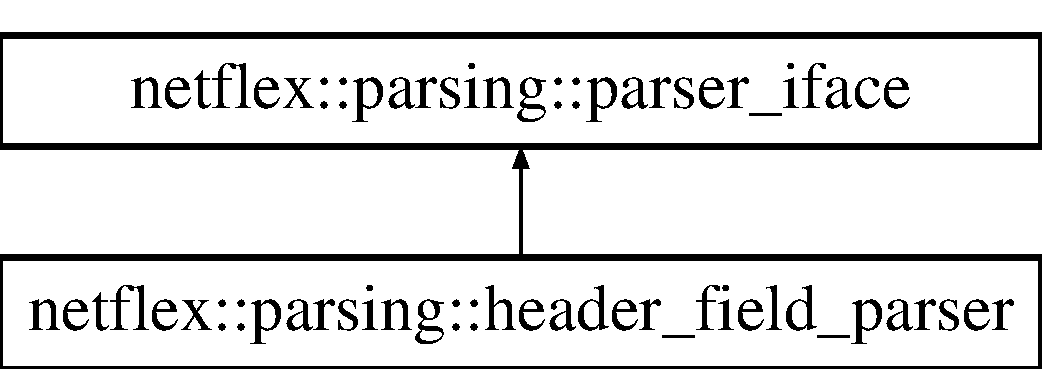
\includegraphics[height=2.000000cm]{classnetflex_1_1parsing_1_1header__field__parser}
\end{center}
\end{figure}
\subsection*{Public Member Functions}
\begin{DoxyCompactItemize}
\item 
\hyperlink{classnetflex_1_1parsing_1_1header__field__parser_a619dc1b993b03073151e3793f2b91bb8}{header\+\_\+field\+\_\+parser} (\hyperlink{classnetflex_1_1http_1_1request}{http\+::request} \&request)
\item 
\hyperlink{classnetflex_1_1parsing_1_1header__field__parser_aa60216c4b9e8c53448402a9cdaf5c495}{$\sim$header\+\_\+field\+\_\+parser} (void)=default
\item 
\mbox{\Hypertarget{classnetflex_1_1parsing_1_1header__field__parser_ad98f22575070c9e2049fae7a39c8b195}\label{classnetflex_1_1parsing_1_1header__field__parser_ad98f22575070c9e2049fae7a39c8b195}} 
\hyperlink{classnetflex_1_1parsing_1_1header__field__parser_ad98f22575070c9e2049fae7a39c8b195}{header\+\_\+field\+\_\+parser} (const \hyperlink{classnetflex_1_1parsing_1_1header__field__parser}{header\+\_\+field\+\_\+parser} \&)=delete
\begin{DoxyCompactList}\small\item\em copy ctor \end{DoxyCompactList}\item 
\mbox{\Hypertarget{classnetflex_1_1parsing_1_1header__field__parser_ac34cdac6009d810413b3e7ba3df9dd96}\label{classnetflex_1_1parsing_1_1header__field__parser_ac34cdac6009d810413b3e7ba3df9dd96}} 
\hyperlink{classnetflex_1_1parsing_1_1header__field__parser}{header\+\_\+field\+\_\+parser} \& \hyperlink{classnetflex_1_1parsing_1_1header__field__parser_ac34cdac6009d810413b3e7ba3df9dd96}{operator=} (const \hyperlink{classnetflex_1_1parsing_1_1header__field__parser}{header\+\_\+field\+\_\+parser} \&)=delete
\begin{DoxyCompactList}\small\item\em assignment operator \end{DoxyCompactList}\item 
void \hyperlink{classnetflex_1_1parsing_1_1header__field__parser_a8c77c07cd5ec5c4f4c5961359b648768}{reset} (void)
\item 
\hyperlink{classnetflex_1_1parsing_1_1parser__iface}{parser\+\_\+iface} \& \hyperlink{classnetflex_1_1parsing_1_1header__field__parser_a9b8f37ee50747394ff9740f36b6ac150}{operator$<$$<$} (std\+::string \&data)
\item 
bool \hyperlink{classnetflex_1_1parsing_1_1header__field__parser_a59cc97a4d2104217d23a4d54a31f072f}{is\+\_\+done} (void) const
\end{DoxyCompactItemize}
\subsection*{Additional Inherited Members}


\subsection{Detailed Description}
parser for a single header field 

\subsection{Constructor \& Destructor Documentation}
\mbox{\Hypertarget{classnetflex_1_1parsing_1_1header__field__parser_a619dc1b993b03073151e3793f2b91bb8}\label{classnetflex_1_1parsing_1_1header__field__parser_a619dc1b993b03073151e3793f2b91bb8}} 
\index{netflex\+::parsing\+::header\+\_\+field\+\_\+parser@{netflex\+::parsing\+::header\+\_\+field\+\_\+parser}!header\+\_\+field\+\_\+parser@{header\+\_\+field\+\_\+parser}}
\index{header\+\_\+field\+\_\+parser@{header\+\_\+field\+\_\+parser}!netflex\+::parsing\+::header\+\_\+field\+\_\+parser@{netflex\+::parsing\+::header\+\_\+field\+\_\+parser}}
\subsubsection{\texorpdfstring{header\+\_\+field\+\_\+parser()}{header\_field\_parser()}}
{\footnotesize\ttfamily netflex\+::parsing\+::header\+\_\+field\+\_\+parser\+::header\+\_\+field\+\_\+parser (\begin{DoxyParamCaption}\item[{\hyperlink{classnetflex_1_1http_1_1request}{http\+::request} \&}]{request }\end{DoxyParamCaption})\hspace{0.3cm}{\ttfamily [explicit]}}

default ctor


\begin{DoxyParams}{Parameters}
{\em request} & request to be initialized \\
\hline
\end{DoxyParams}
\mbox{\Hypertarget{classnetflex_1_1parsing_1_1header__field__parser_aa60216c4b9e8c53448402a9cdaf5c495}\label{classnetflex_1_1parsing_1_1header__field__parser_aa60216c4b9e8c53448402a9cdaf5c495}} 
\index{netflex\+::parsing\+::header\+\_\+field\+\_\+parser@{netflex\+::parsing\+::header\+\_\+field\+\_\+parser}!````~header\+\_\+field\+\_\+parser@{$\sim$header\+\_\+field\+\_\+parser}}
\index{````~header\+\_\+field\+\_\+parser@{$\sim$header\+\_\+field\+\_\+parser}!netflex\+::parsing\+::header\+\_\+field\+\_\+parser@{netflex\+::parsing\+::header\+\_\+field\+\_\+parser}}
\subsubsection{\texorpdfstring{$\sim$header\+\_\+field\+\_\+parser()}{~header\_field\_parser()}}
{\footnotesize\ttfamily netflex\+::parsing\+::header\+\_\+field\+\_\+parser\+::$\sim$header\+\_\+field\+\_\+parser (\begin{DoxyParamCaption}\item[{void}]{ }\end{DoxyParamCaption})\hspace{0.3cm}{\ttfamily [default]}}

default dtor 

\subsection{Member Function Documentation}
\mbox{\Hypertarget{classnetflex_1_1parsing_1_1header__field__parser_a59cc97a4d2104217d23a4d54a31f072f}\label{classnetflex_1_1parsing_1_1header__field__parser_a59cc97a4d2104217d23a4d54a31f072f}} 
\index{netflex\+::parsing\+::header\+\_\+field\+\_\+parser@{netflex\+::parsing\+::header\+\_\+field\+\_\+parser}!is\+\_\+done@{is\+\_\+done}}
\index{is\+\_\+done@{is\+\_\+done}!netflex\+::parsing\+::header\+\_\+field\+\_\+parser@{netflex\+::parsing\+::header\+\_\+field\+\_\+parser}}
\subsubsection{\texorpdfstring{is\+\_\+done()}{is\_done()}}
{\footnotesize\ttfamily bool netflex\+::parsing\+::header\+\_\+field\+\_\+parser\+::is\+\_\+done (\begin{DoxyParamCaption}\item[{void}]{ }\end{DoxyParamCaption}) const\hspace{0.3cm}{\ttfamily [virtual]}}

\begin{DoxyReturn}{Returns}
whether the parsing is done or not 
\end{DoxyReturn}


Implements \hyperlink{classnetflex_1_1parsing_1_1parser__iface_afebd1cc50d5958f712dfac0c023fd162}{netflex\+::parsing\+::parser\+\_\+iface}.

\mbox{\Hypertarget{classnetflex_1_1parsing_1_1header__field__parser_a9b8f37ee50747394ff9740f36b6ac150}\label{classnetflex_1_1parsing_1_1header__field__parser_a9b8f37ee50747394ff9740f36b6ac150}} 
\index{netflex\+::parsing\+::header\+\_\+field\+\_\+parser@{netflex\+::parsing\+::header\+\_\+field\+\_\+parser}!operator$<$$<$@{operator$<$$<$}}
\index{operator$<$$<$@{operator$<$$<$}!netflex\+::parsing\+::header\+\_\+field\+\_\+parser@{netflex\+::parsing\+::header\+\_\+field\+\_\+parser}}
\subsubsection{\texorpdfstring{operator$<$$<$()}{operator<<()}}
{\footnotesize\ttfamily \hyperlink{classnetflex_1_1parsing_1_1parser__iface}{parser\+\_\+iface}\& netflex\+::parsing\+::header\+\_\+field\+\_\+parser\+::operator$<$$<$ (\begin{DoxyParamCaption}\item[{std\+::string \&}]{data }\end{DoxyParamCaption})\hspace{0.3cm}{\ttfamily [virtual]}}

consume input data to parse it and init the request if not enough data is passed in, this method would need to be called again later input data is modified whenever a token is consumed by parsing, even if parsing is incomplete or invalid invalid data would lead to a raised exception


\begin{DoxyParams}{Parameters}
{\em data} & input data to be parsed \\
\hline
\end{DoxyParams}
\begin{DoxyReturn}{Returns}
reference to the current object 
\end{DoxyReturn}


Implements \hyperlink{classnetflex_1_1parsing_1_1parser__iface_a6b092567e70a5c0bf7568e94d06f7154}{netflex\+::parsing\+::parser\+\_\+iface}.

\mbox{\Hypertarget{classnetflex_1_1parsing_1_1header__field__parser_a8c77c07cd5ec5c4f4c5961359b648768}\label{classnetflex_1_1parsing_1_1header__field__parser_a8c77c07cd5ec5c4f4c5961359b648768}} 
\index{netflex\+::parsing\+::header\+\_\+field\+\_\+parser@{netflex\+::parsing\+::header\+\_\+field\+\_\+parser}!reset@{reset}}
\index{reset@{reset}!netflex\+::parsing\+::header\+\_\+field\+\_\+parser@{netflex\+::parsing\+::header\+\_\+field\+\_\+parser}}
\subsubsection{\texorpdfstring{reset()}{reset()}}
{\footnotesize\ttfamily void netflex\+::parsing\+::header\+\_\+field\+\_\+parser\+::reset (\begin{DoxyParamCaption}\item[{void}]{ }\end{DoxyParamCaption})}

reset state of parsing (startover again) 

The documentation for this class was generated from the following file\+:\begin{DoxyCompactItemize}
\item 
includes/netflex/parsing/header\+\_\+field\+\_\+parser.\+hpp\end{DoxyCompactItemize}

\hypertarget{classnetflex_1_1parsing_1_1header__fields__parser}{}\section{netflex\+:\+:parsing\+:\+:header\+\_\+fields\+\_\+parser Class Reference}
\label{classnetflex_1_1parsing_1_1header__fields__parser}\index{netflex\+::parsing\+::header\+\_\+fields\+\_\+parser@{netflex\+::parsing\+::header\+\_\+fields\+\_\+parser}}


{\ttfamily \#include $<$header\+\_\+fields\+\_\+parser.\+hpp$>$}

Inheritance diagram for netflex\+:\+:parsing\+:\+:header\+\_\+fields\+\_\+parser\+:\begin{figure}[H]
\begin{center}
\leavevmode
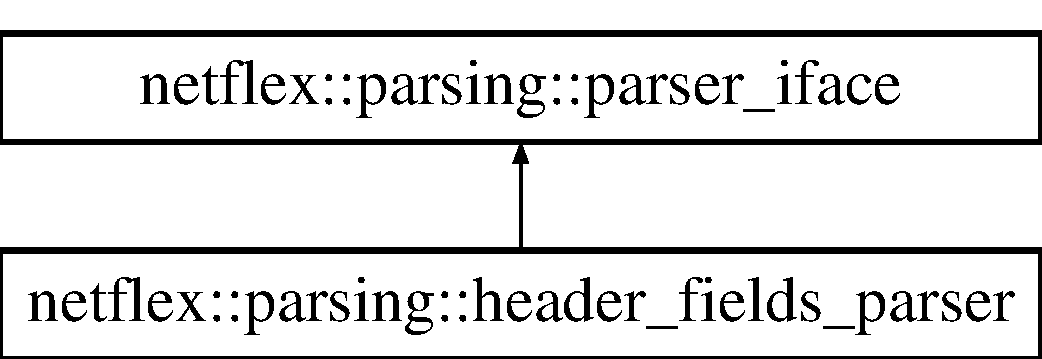
\includegraphics[height=2.000000cm]{classnetflex_1_1parsing_1_1header__fields__parser}
\end{center}
\end{figure}
\subsection*{Public Member Functions}
\begin{DoxyCompactItemize}
\item 
\hyperlink{classnetflex_1_1parsing_1_1header__fields__parser_a062871b585ec94f1ef3039237debfd4f}{header\+\_\+fields\+\_\+parser} (\hyperlink{classnetflex_1_1http_1_1request}{http\+::request} \&request)
\item 
\mbox{\Hypertarget{classnetflex_1_1parsing_1_1header__fields__parser_ae6497c8612a0200de763a5b91c574398}\label{classnetflex_1_1parsing_1_1header__fields__parser_ae6497c8612a0200de763a5b91c574398}} 
\hyperlink{classnetflex_1_1parsing_1_1header__fields__parser_ae6497c8612a0200de763a5b91c574398}{$\sim$header\+\_\+fields\+\_\+parser} (void)=default
\begin{DoxyCompactList}\small\item\em default dtor \end{DoxyCompactList}\item 
\mbox{\Hypertarget{classnetflex_1_1parsing_1_1header__fields__parser_a09177036c57944df36217a024e64de3f}\label{classnetflex_1_1parsing_1_1header__fields__parser_a09177036c57944df36217a024e64de3f}} 
\hyperlink{classnetflex_1_1parsing_1_1header__fields__parser_a09177036c57944df36217a024e64de3f}{header\+\_\+fields\+\_\+parser} (const \hyperlink{classnetflex_1_1parsing_1_1header__fields__parser}{header\+\_\+fields\+\_\+parser} \&)=delete
\begin{DoxyCompactList}\small\item\em copy ctor \end{DoxyCompactList}\item 
\mbox{\Hypertarget{classnetflex_1_1parsing_1_1header__fields__parser_aebe26ebcd6cccc0e010eaa82a2173d91}\label{classnetflex_1_1parsing_1_1header__fields__parser_aebe26ebcd6cccc0e010eaa82a2173d91}} 
\hyperlink{classnetflex_1_1parsing_1_1header__fields__parser}{header\+\_\+fields\+\_\+parser} \& \hyperlink{classnetflex_1_1parsing_1_1header__fields__parser_aebe26ebcd6cccc0e010eaa82a2173d91}{operator=} (const \hyperlink{classnetflex_1_1parsing_1_1header__fields__parser}{header\+\_\+fields\+\_\+parser} \&)=delete
\begin{DoxyCompactList}\small\item\em assignment operator \end{DoxyCompactList}\item 
\hyperlink{classnetflex_1_1parsing_1_1parser__iface}{parser\+\_\+iface} \& \hyperlink{classnetflex_1_1parsing_1_1header__fields__parser_a4ba3f5dad38f3f9ef9bf3632f02d4111}{operator$<$$<$} (std\+::string \&data)
\item 
bool \hyperlink{classnetflex_1_1parsing_1_1header__fields__parser_a8303c3f2910b9baa68b9b0313e0438cf}{is\+\_\+done} (void) const
\end{DoxyCompactItemize}
\subsection*{Additional Inherited Members}


\subsection{Detailed Description}
parser for all header fields 

\subsection{Constructor \& Destructor Documentation}
\mbox{\Hypertarget{classnetflex_1_1parsing_1_1header__fields__parser_a062871b585ec94f1ef3039237debfd4f}\label{classnetflex_1_1parsing_1_1header__fields__parser_a062871b585ec94f1ef3039237debfd4f}} 
\index{netflex\+::parsing\+::header\+\_\+fields\+\_\+parser@{netflex\+::parsing\+::header\+\_\+fields\+\_\+parser}!header\+\_\+fields\+\_\+parser@{header\+\_\+fields\+\_\+parser}}
\index{header\+\_\+fields\+\_\+parser@{header\+\_\+fields\+\_\+parser}!netflex\+::parsing\+::header\+\_\+fields\+\_\+parser@{netflex\+::parsing\+::header\+\_\+fields\+\_\+parser}}
\subsubsection{\texorpdfstring{header\+\_\+fields\+\_\+parser()}{header\_fields\_parser()}}
{\footnotesize\ttfamily netflex\+::parsing\+::header\+\_\+fields\+\_\+parser\+::header\+\_\+fields\+\_\+parser (\begin{DoxyParamCaption}\item[{\hyperlink{classnetflex_1_1http_1_1request}{http\+::request} \&}]{request }\end{DoxyParamCaption})\hspace{0.3cm}{\ttfamily [explicit]}}

default ctor


\begin{DoxyParams}{Parameters}
{\em request} & request to be initialized \\
\hline
\end{DoxyParams}


\subsection{Member Function Documentation}
\mbox{\Hypertarget{classnetflex_1_1parsing_1_1header__fields__parser_a8303c3f2910b9baa68b9b0313e0438cf}\label{classnetflex_1_1parsing_1_1header__fields__parser_a8303c3f2910b9baa68b9b0313e0438cf}} 
\index{netflex\+::parsing\+::header\+\_\+fields\+\_\+parser@{netflex\+::parsing\+::header\+\_\+fields\+\_\+parser}!is\+\_\+done@{is\+\_\+done}}
\index{is\+\_\+done@{is\+\_\+done}!netflex\+::parsing\+::header\+\_\+fields\+\_\+parser@{netflex\+::parsing\+::header\+\_\+fields\+\_\+parser}}
\subsubsection{\texorpdfstring{is\+\_\+done()}{is\_done()}}
{\footnotesize\ttfamily bool netflex\+::parsing\+::header\+\_\+fields\+\_\+parser\+::is\+\_\+done (\begin{DoxyParamCaption}\item[{void}]{ }\end{DoxyParamCaption}) const\hspace{0.3cm}{\ttfamily [virtual]}}

\begin{DoxyReturn}{Returns}
whether the parsing is done or not 
\end{DoxyReturn}


Implements \hyperlink{classnetflex_1_1parsing_1_1parser__iface_afebd1cc50d5958f712dfac0c023fd162}{netflex\+::parsing\+::parser\+\_\+iface}.

\mbox{\Hypertarget{classnetflex_1_1parsing_1_1header__fields__parser_a4ba3f5dad38f3f9ef9bf3632f02d4111}\label{classnetflex_1_1parsing_1_1header__fields__parser_a4ba3f5dad38f3f9ef9bf3632f02d4111}} 
\index{netflex\+::parsing\+::header\+\_\+fields\+\_\+parser@{netflex\+::parsing\+::header\+\_\+fields\+\_\+parser}!operator$<$$<$@{operator$<$$<$}}
\index{operator$<$$<$@{operator$<$$<$}!netflex\+::parsing\+::header\+\_\+fields\+\_\+parser@{netflex\+::parsing\+::header\+\_\+fields\+\_\+parser}}
\subsubsection{\texorpdfstring{operator$<$$<$()}{operator<<()}}
{\footnotesize\ttfamily \hyperlink{classnetflex_1_1parsing_1_1parser__iface}{parser\+\_\+iface}\& netflex\+::parsing\+::header\+\_\+fields\+\_\+parser\+::operator$<$$<$ (\begin{DoxyParamCaption}\item[{std\+::string \&}]{data }\end{DoxyParamCaption})\hspace{0.3cm}{\ttfamily [virtual]}}

consume input data to parse it and init the request if not enough data is passed in, this method would need to be called again later input data is modified whenever a token is consumed by parsing, even if parsing is incomplete or invalid invalid data would lead to a raised exception


\begin{DoxyParams}{Parameters}
{\em data} & input data to be parsed \\
\hline
\end{DoxyParams}
\begin{DoxyReturn}{Returns}
reference to the current object 
\end{DoxyReturn}


Implements \hyperlink{classnetflex_1_1parsing_1_1parser__iface_a6b092567e70a5c0bf7568e94d06f7154}{netflex\+::parsing\+::parser\+\_\+iface}.



The documentation for this class was generated from the following file\+:\begin{DoxyCompactItemize}
\item 
includes/netflex/parsing/header\+\_\+fields\+\_\+parser.\+hpp\end{DoxyCompactItemize}

\hypertarget{classnetflex_1_1logger}{}\section{netflex\+:\+:logger Class Reference}
\label{classnetflex_1_1logger}\index{netflex\+::logger@{netflex\+::logger}}


{\ttfamily \#include $<$logger.\+hpp$>$}

Inheritance diagram for netflex\+:\+:logger\+:\begin{figure}[H]
\begin{center}
\leavevmode
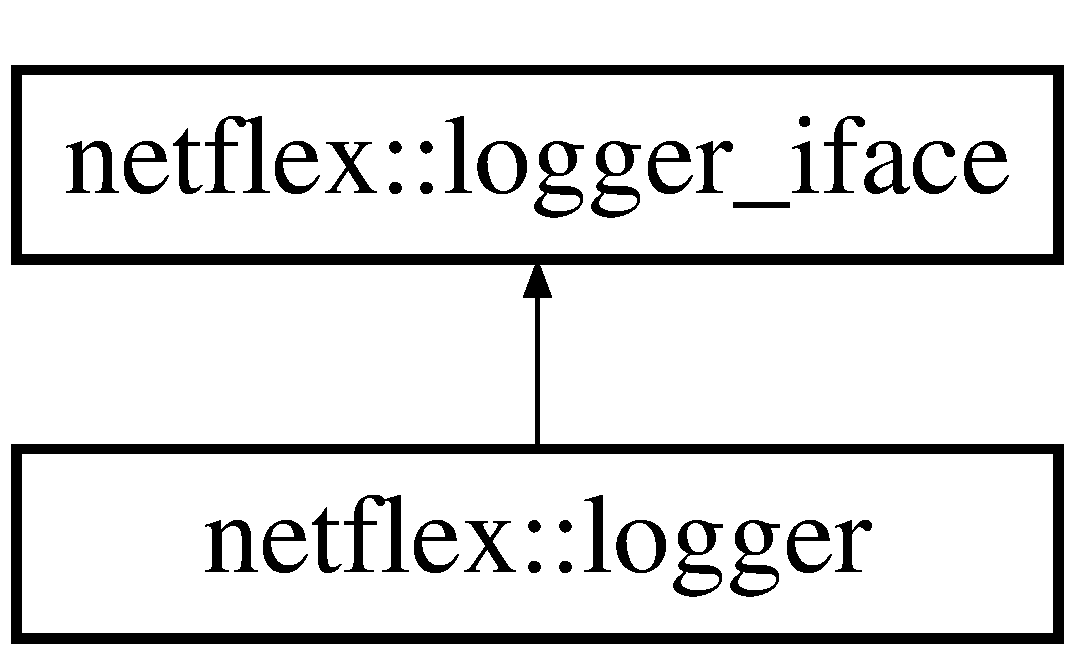
\includegraphics[height=2.000000cm]{classnetflex_1_1logger}
\end{center}
\end{figure}
\subsection*{Public Types}
\begin{DoxyCompactItemize}
\item 
enum \hyperlink{classnetflex_1_1logger_a8270276b1351480a8a9bfab4139cdc9c}{log\+\_\+level} \{ {\bfseries error} = 0, 
{\bfseries warn} = 1, 
{\bfseries info} = 2, 
{\bfseries debug} = 3
 \}
\end{DoxyCompactItemize}
\subsection*{Public Member Functions}
\begin{DoxyCompactItemize}
\item 
\mbox{\Hypertarget{classnetflex_1_1logger_a8ed6f964305456a251c83761d5da70a7}\label{classnetflex_1_1logger_a8ed6f964305456a251c83761d5da70a7}} 
\hyperlink{classnetflex_1_1logger_a8ed6f964305456a251c83761d5da70a7}{logger} (\hyperlink{classnetflex_1_1logger_a8270276b1351480a8a9bfab4139cdc9c}{log\+\_\+level} level=log\+\_\+level\+::info)
\begin{DoxyCompactList}\small\item\em ctor \end{DoxyCompactList}\item 
\mbox{\Hypertarget{classnetflex_1_1logger_a93c7908219e8d992f7eb52b133b9b23a}\label{classnetflex_1_1logger_a93c7908219e8d992f7eb52b133b9b23a}} 
\hyperlink{classnetflex_1_1logger_a93c7908219e8d992f7eb52b133b9b23a}{$\sim$logger} (void)=default
\begin{DoxyCompactList}\small\item\em dtor \end{DoxyCompactList}\item 
\mbox{\Hypertarget{classnetflex_1_1logger_ac4f3c65364cfc45034cec215d518afdf}\label{classnetflex_1_1logger_ac4f3c65364cfc45034cec215d518afdf}} 
\hyperlink{classnetflex_1_1logger_ac4f3c65364cfc45034cec215d518afdf}{logger} (const \hyperlink{classnetflex_1_1logger}{logger} \&)=default
\begin{DoxyCompactList}\small\item\em copy ctor \end{DoxyCompactList}\item 
\mbox{\Hypertarget{classnetflex_1_1logger_ac709fc0f8713f94795031e555fab7afb}\label{classnetflex_1_1logger_ac709fc0f8713f94795031e555fab7afb}} 
\hyperlink{classnetflex_1_1logger}{logger} \& \hyperlink{classnetflex_1_1logger_ac709fc0f8713f94795031e555fab7afb}{operator=} (const \hyperlink{classnetflex_1_1logger}{logger} \&)=default
\begin{DoxyCompactList}\small\item\em assignment operator \end{DoxyCompactList}\item 
void \hyperlink{classnetflex_1_1logger_a6acb4c370bbacf855ec9e039defdb39c}{debug} (const std\+::string \&msg, const std\+::string \&file, std\+::size\+\_\+t line)
\item 
void \hyperlink{classnetflex_1_1logger_a5663c09b0fddff8efcc8556bc600bff4}{info} (const std\+::string \&msg, const std\+::string \&file, std\+::size\+\_\+t line)
\item 
void \hyperlink{classnetflex_1_1logger_a0874f423d630a7263fd89ce6a2e3c2f9}{warn} (const std\+::string \&msg, const std\+::string \&file, std\+::size\+\_\+t line)
\item 
void \hyperlink{classnetflex_1_1logger_a1692266cfb80ea4e1f77f4d28a377875}{error} (const std\+::string \&msg, const std\+::string \&file, std\+::size\+\_\+t line)
\end{DoxyCompactItemize}


\subsection{Detailed Description}
default logger class provided by the library 

\subsection{Member Enumeration Documentation}
\mbox{\Hypertarget{classnetflex_1_1logger_a8270276b1351480a8a9bfab4139cdc9c}\label{classnetflex_1_1logger_a8270276b1351480a8a9bfab4139cdc9c}} 
\index{netflex\+::logger@{netflex\+::logger}!log\+\_\+level@{log\+\_\+level}}
\index{log\+\_\+level@{log\+\_\+level}!netflex\+::logger@{netflex\+::logger}}
\subsubsection{\texorpdfstring{log\+\_\+level}{log\_level}}
{\footnotesize\ttfamily enum \hyperlink{classnetflex_1_1logger_a8270276b1351480a8a9bfab4139cdc9c}{netflex\+::logger\+::log\+\_\+level}\hspace{0.3cm}{\ttfamily [strong]}}

log level 

\subsection{Member Function Documentation}
\mbox{\Hypertarget{classnetflex_1_1logger_a6acb4c370bbacf855ec9e039defdb39c}\label{classnetflex_1_1logger_a6acb4c370bbacf855ec9e039defdb39c}} 
\index{netflex\+::logger@{netflex\+::logger}!debug@{debug}}
\index{debug@{debug}!netflex\+::logger@{netflex\+::logger}}
\subsubsection{\texorpdfstring{debug()}{debug()}}
{\footnotesize\ttfamily void netflex\+::logger\+::debug (\begin{DoxyParamCaption}\item[{const std\+::string \&}]{msg,  }\item[{const std\+::string \&}]{file,  }\item[{std\+::size\+\_\+t}]{line }\end{DoxyParamCaption})\hspace{0.3cm}{\ttfamily [virtual]}}

debug logging


\begin{DoxyParams}{Parameters}
{\em msg} & message to be logged \\
\hline
{\em file} & file from which the message is coming \\
\hline
{\em line} & line in the file of the message \\
\hline
\end{DoxyParams}


Implements \hyperlink{classnetflex_1_1logger__iface_a0768fd1687f7d449b0cde0058038d52a}{netflex\+::logger\+\_\+iface}.

\mbox{\Hypertarget{classnetflex_1_1logger_a1692266cfb80ea4e1f77f4d28a377875}\label{classnetflex_1_1logger_a1692266cfb80ea4e1f77f4d28a377875}} 
\index{netflex\+::logger@{netflex\+::logger}!error@{error}}
\index{error@{error}!netflex\+::logger@{netflex\+::logger}}
\subsubsection{\texorpdfstring{error()}{error()}}
{\footnotesize\ttfamily void netflex\+::logger\+::error (\begin{DoxyParamCaption}\item[{const std\+::string \&}]{msg,  }\item[{const std\+::string \&}]{file,  }\item[{std\+::size\+\_\+t}]{line }\end{DoxyParamCaption})\hspace{0.3cm}{\ttfamily [virtual]}}

error logging


\begin{DoxyParams}{Parameters}
{\em msg} & message to be logged \\
\hline
{\em file} & file from which the message is coming \\
\hline
{\em line} & line in the file of the message \\
\hline
\end{DoxyParams}


Implements \hyperlink{classnetflex_1_1logger__iface_a09e4dda02d64e420cf0d91cbef00fe1c}{netflex\+::logger\+\_\+iface}.

\mbox{\Hypertarget{classnetflex_1_1logger_a5663c09b0fddff8efcc8556bc600bff4}\label{classnetflex_1_1logger_a5663c09b0fddff8efcc8556bc600bff4}} 
\index{netflex\+::logger@{netflex\+::logger}!info@{info}}
\index{info@{info}!netflex\+::logger@{netflex\+::logger}}
\subsubsection{\texorpdfstring{info()}{info()}}
{\footnotesize\ttfamily void netflex\+::logger\+::info (\begin{DoxyParamCaption}\item[{const std\+::string \&}]{msg,  }\item[{const std\+::string \&}]{file,  }\item[{std\+::size\+\_\+t}]{line }\end{DoxyParamCaption})\hspace{0.3cm}{\ttfamily [virtual]}}

info logging


\begin{DoxyParams}{Parameters}
{\em msg} & message to be logged \\
\hline
{\em file} & file from which the message is coming \\
\hline
{\em line} & line in the file of the message \\
\hline
\end{DoxyParams}


Implements \hyperlink{classnetflex_1_1logger__iface_aac8e95dd5c24ac109e33c0002be110f0}{netflex\+::logger\+\_\+iface}.

\mbox{\Hypertarget{classnetflex_1_1logger_a0874f423d630a7263fd89ce6a2e3c2f9}\label{classnetflex_1_1logger_a0874f423d630a7263fd89ce6a2e3c2f9}} 
\index{netflex\+::logger@{netflex\+::logger}!warn@{warn}}
\index{warn@{warn}!netflex\+::logger@{netflex\+::logger}}
\subsubsection{\texorpdfstring{warn()}{warn()}}
{\footnotesize\ttfamily void netflex\+::logger\+::warn (\begin{DoxyParamCaption}\item[{const std\+::string \&}]{msg,  }\item[{const std\+::string \&}]{file,  }\item[{std\+::size\+\_\+t}]{line }\end{DoxyParamCaption})\hspace{0.3cm}{\ttfamily [virtual]}}

warn logging


\begin{DoxyParams}{Parameters}
{\em msg} & message to be logged \\
\hline
{\em file} & file from which the message is coming \\
\hline
{\em line} & line in the file of the message \\
\hline
\end{DoxyParams}


Implements \hyperlink{classnetflex_1_1logger__iface_a0d1ee72c9b5ba9f08cb306d69ecc4822}{netflex\+::logger\+\_\+iface}.



The documentation for this class was generated from the following file\+:\begin{DoxyCompactItemize}
\item 
includes/netflex/misc/logger.\+hpp\end{DoxyCompactItemize}

\hypertarget{classnetflex_1_1logger__iface}{}\section{netflex\+:\+:logger\+\_\+iface Class Reference}
\label{classnetflex_1_1logger__iface}\index{netflex\+::logger\+\_\+iface@{netflex\+::logger\+\_\+iface}}


{\ttfamily \#include $<$logger.\+hpp$>$}

Inheritance diagram for netflex\+:\+:logger\+\_\+iface\+:\begin{figure}[H]
\begin{center}
\leavevmode
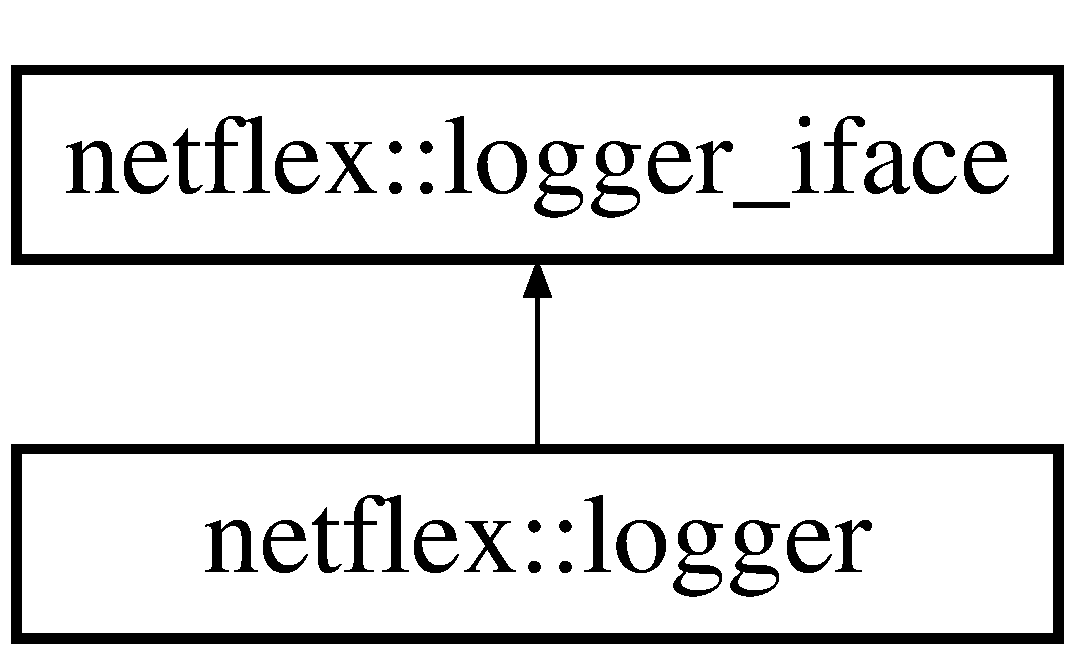
\includegraphics[height=2.000000cm]{classnetflex_1_1logger__iface}
\end{center}
\end{figure}
\subsection*{Public Member Functions}
\begin{DoxyCompactItemize}
\item 
\mbox{\Hypertarget{classnetflex_1_1logger__iface_a905b0aa24d0f482fb6bf92ebfcb1babb}\label{classnetflex_1_1logger__iface_a905b0aa24d0f482fb6bf92ebfcb1babb}} 
\hyperlink{classnetflex_1_1logger__iface_a905b0aa24d0f482fb6bf92ebfcb1babb}{logger\+\_\+iface} (void)=default
\begin{DoxyCompactList}\small\item\em ctor \end{DoxyCompactList}\item 
\mbox{\Hypertarget{classnetflex_1_1logger__iface_a47532b28d85ac8acb08cf0354f15262d}\label{classnetflex_1_1logger__iface_a47532b28d85ac8acb08cf0354f15262d}} 
virtual \hyperlink{classnetflex_1_1logger__iface_a47532b28d85ac8acb08cf0354f15262d}{$\sim$logger\+\_\+iface} (void)=default
\begin{DoxyCompactList}\small\item\em dtor \end{DoxyCompactList}\item 
\mbox{\Hypertarget{classnetflex_1_1logger__iface_a761fb0e8a80fbb28a73a9e216230b64d}\label{classnetflex_1_1logger__iface_a761fb0e8a80fbb28a73a9e216230b64d}} 
\hyperlink{classnetflex_1_1logger__iface_a761fb0e8a80fbb28a73a9e216230b64d}{logger\+\_\+iface} (const \hyperlink{classnetflex_1_1logger__iface}{logger\+\_\+iface} \&)=default
\begin{DoxyCompactList}\small\item\em copy ctor \end{DoxyCompactList}\item 
\mbox{\Hypertarget{classnetflex_1_1logger__iface_a966026574277bb4910d83d13b872aa68}\label{classnetflex_1_1logger__iface_a966026574277bb4910d83d13b872aa68}} 
\hyperlink{classnetflex_1_1logger__iface}{logger\+\_\+iface} \& \hyperlink{classnetflex_1_1logger__iface_a966026574277bb4910d83d13b872aa68}{operator=} (const \hyperlink{classnetflex_1_1logger__iface}{logger\+\_\+iface} \&)=default
\begin{DoxyCompactList}\small\item\em assignment operator \end{DoxyCompactList}\item 
virtual void \hyperlink{classnetflex_1_1logger__iface_a0768fd1687f7d449b0cde0058038d52a}{debug} (const std\+::string \&msg, const std\+::string \&file, std\+::size\+\_\+t line)=0
\item 
virtual void \hyperlink{classnetflex_1_1logger__iface_aac8e95dd5c24ac109e33c0002be110f0}{info} (const std\+::string \&msg, const std\+::string \&file, std\+::size\+\_\+t line)=0
\item 
virtual void \hyperlink{classnetflex_1_1logger__iface_a0d1ee72c9b5ba9f08cb306d69ecc4822}{warn} (const std\+::string \&msg, const std\+::string \&file, std\+::size\+\_\+t line)=0
\item 
virtual void \hyperlink{classnetflex_1_1logger__iface_a09e4dda02d64e420cf0d91cbef00fe1c}{error} (const std\+::string \&msg, const std\+::string \&file, std\+::size\+\_\+t line)=0
\end{DoxyCompactItemize}


\subsection{Detailed Description}
\hyperlink{classnetflex_1_1logger__iface}{logger\+\_\+iface} should be inherited by any class intended to be used for logging 

\subsection{Member Function Documentation}
\mbox{\Hypertarget{classnetflex_1_1logger__iface_a0768fd1687f7d449b0cde0058038d52a}\label{classnetflex_1_1logger__iface_a0768fd1687f7d449b0cde0058038d52a}} 
\index{netflex\+::logger\+\_\+iface@{netflex\+::logger\+\_\+iface}!debug@{debug}}
\index{debug@{debug}!netflex\+::logger\+\_\+iface@{netflex\+::logger\+\_\+iface}}
\subsubsection{\texorpdfstring{debug()}{debug()}}
{\footnotesize\ttfamily virtual void netflex\+::logger\+\_\+iface\+::debug (\begin{DoxyParamCaption}\item[{const std\+::string \&}]{msg,  }\item[{const std\+::string \&}]{file,  }\item[{std\+::size\+\_\+t}]{line }\end{DoxyParamCaption})\hspace{0.3cm}{\ttfamily [pure virtual]}}

debug logging


\begin{DoxyParams}{Parameters}
{\em msg} & message to be logged \\
\hline
{\em file} & file from which the message is coming \\
\hline
{\em line} & line in the file of the message \\
\hline
\end{DoxyParams}


Implemented in \hyperlink{classnetflex_1_1logger_a6acb4c370bbacf855ec9e039defdb39c}{netflex\+::logger}.

\mbox{\Hypertarget{classnetflex_1_1logger__iface_a09e4dda02d64e420cf0d91cbef00fe1c}\label{classnetflex_1_1logger__iface_a09e4dda02d64e420cf0d91cbef00fe1c}} 
\index{netflex\+::logger\+\_\+iface@{netflex\+::logger\+\_\+iface}!error@{error}}
\index{error@{error}!netflex\+::logger\+\_\+iface@{netflex\+::logger\+\_\+iface}}
\subsubsection{\texorpdfstring{error()}{error()}}
{\footnotesize\ttfamily virtual void netflex\+::logger\+\_\+iface\+::error (\begin{DoxyParamCaption}\item[{const std\+::string \&}]{msg,  }\item[{const std\+::string \&}]{file,  }\item[{std\+::size\+\_\+t}]{line }\end{DoxyParamCaption})\hspace{0.3cm}{\ttfamily [pure virtual]}}

error logging


\begin{DoxyParams}{Parameters}
{\em msg} & message to be logged \\
\hline
{\em file} & file from which the message is coming \\
\hline
{\em line} & line in the file of the message \\
\hline
\end{DoxyParams}


Implemented in \hyperlink{classnetflex_1_1logger_a1692266cfb80ea4e1f77f4d28a377875}{netflex\+::logger}.

\mbox{\Hypertarget{classnetflex_1_1logger__iface_aac8e95dd5c24ac109e33c0002be110f0}\label{classnetflex_1_1logger__iface_aac8e95dd5c24ac109e33c0002be110f0}} 
\index{netflex\+::logger\+\_\+iface@{netflex\+::logger\+\_\+iface}!info@{info}}
\index{info@{info}!netflex\+::logger\+\_\+iface@{netflex\+::logger\+\_\+iface}}
\subsubsection{\texorpdfstring{info()}{info()}}
{\footnotesize\ttfamily virtual void netflex\+::logger\+\_\+iface\+::info (\begin{DoxyParamCaption}\item[{const std\+::string \&}]{msg,  }\item[{const std\+::string \&}]{file,  }\item[{std\+::size\+\_\+t}]{line }\end{DoxyParamCaption})\hspace{0.3cm}{\ttfamily [pure virtual]}}

info logging


\begin{DoxyParams}{Parameters}
{\em msg} & message to be logged \\
\hline
{\em file} & file from which the message is coming \\
\hline
{\em line} & line in the file of the message \\
\hline
\end{DoxyParams}


Implemented in \hyperlink{classnetflex_1_1logger_a5663c09b0fddff8efcc8556bc600bff4}{netflex\+::logger}.

\mbox{\Hypertarget{classnetflex_1_1logger__iface_a0d1ee72c9b5ba9f08cb306d69ecc4822}\label{classnetflex_1_1logger__iface_a0d1ee72c9b5ba9f08cb306d69ecc4822}} 
\index{netflex\+::logger\+\_\+iface@{netflex\+::logger\+\_\+iface}!warn@{warn}}
\index{warn@{warn}!netflex\+::logger\+\_\+iface@{netflex\+::logger\+\_\+iface}}
\subsubsection{\texorpdfstring{warn()}{warn()}}
{\footnotesize\ttfamily virtual void netflex\+::logger\+\_\+iface\+::warn (\begin{DoxyParamCaption}\item[{const std\+::string \&}]{msg,  }\item[{const std\+::string \&}]{file,  }\item[{std\+::size\+\_\+t}]{line }\end{DoxyParamCaption})\hspace{0.3cm}{\ttfamily [pure virtual]}}

warn logging


\begin{DoxyParams}{Parameters}
{\em msg} & message to be logged \\
\hline
{\em file} & file from which the message is coming \\
\hline
{\em line} & line in the file of the message \\
\hline
\end{DoxyParams}


Implemented in \hyperlink{classnetflex_1_1logger_a0874f423d630a7263fd89ce6a2e3c2f9}{netflex\+::logger}.



The documentation for this class was generated from the following file\+:\begin{DoxyCompactItemize}
\item 
includes/netflex/misc/logger.\+hpp\end{DoxyCompactItemize}

\hypertarget{classnetflex_1_1parsing_1_1message__body__chuncked__parser}{}\section{netflex\+:\+:parsing\+:\+:message\+\_\+body\+\_\+chuncked\+\_\+parser Class Reference}
\label{classnetflex_1_1parsing_1_1message__body__chuncked__parser}\index{netflex\+::parsing\+::message\+\_\+body\+\_\+chuncked\+\_\+parser@{netflex\+::parsing\+::message\+\_\+body\+\_\+chuncked\+\_\+parser}}
Inheritance diagram for netflex\+:\+:parsing\+:\+:message\+\_\+body\+\_\+chuncked\+\_\+parser\+:\begin{figure}[H]
\begin{center}
\leavevmode
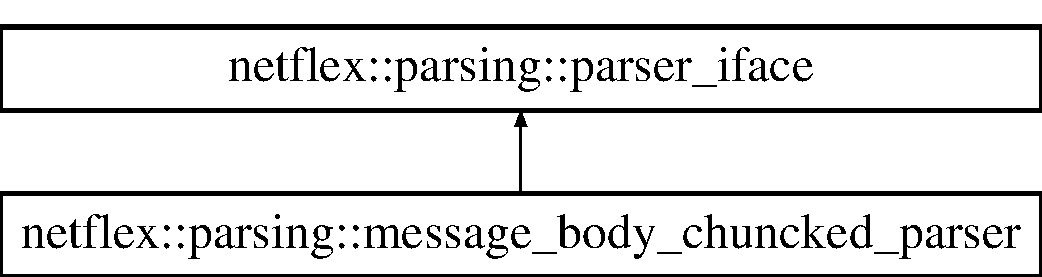
\includegraphics[height=2.000000cm]{classnetflex_1_1parsing_1_1message__body__chuncked__parser}
\end{center}
\end{figure}
\subsection*{Public Member Functions}
\begin{DoxyCompactItemize}
\item 
\mbox{\Hypertarget{classnetflex_1_1parsing_1_1message__body__chuncked__parser_a14516267172bd9388292dab58e2d02f3}\label{classnetflex_1_1parsing_1_1message__body__chuncked__parser_a14516267172bd9388292dab58e2d02f3}} 
\hyperlink{classnetflex_1_1parsing_1_1message__body__chuncked__parser_a14516267172bd9388292dab58e2d02f3}{message\+\_\+body\+\_\+chuncked\+\_\+parser} (\hyperlink{classnetflex_1_1http_1_1request}{http\+::request} \&request)
\begin{DoxyCompactList}\small\item\em ctor \& dtor \end{DoxyCompactList}\item 
\mbox{\Hypertarget{classnetflex_1_1parsing_1_1message__body__chuncked__parser_a9a924a41f4a72833331a0120d2045eaa}\label{classnetflex_1_1parsing_1_1message__body__chuncked__parser_a9a924a41f4a72833331a0120d2045eaa}} 
\hyperlink{classnetflex_1_1parsing_1_1message__body__chuncked__parser_a9a924a41f4a72833331a0120d2045eaa}{message\+\_\+body\+\_\+chuncked\+\_\+parser} (const \hyperlink{classnetflex_1_1parsing_1_1message__body__chuncked__parser}{message\+\_\+body\+\_\+chuncked\+\_\+parser} \&)=delete
\begin{DoxyCompactList}\small\item\em copy ctor \& assignment operator \end{DoxyCompactList}\item 
\mbox{\Hypertarget{classnetflex_1_1parsing_1_1message__body__chuncked__parser_ab10ac43d89941c4521ab9fbba8fab540}\label{classnetflex_1_1parsing_1_1message__body__chuncked__parser_ab10ac43d89941c4521ab9fbba8fab540}} 
\hyperlink{classnetflex_1_1parsing_1_1message__body__chuncked__parser}{message\+\_\+body\+\_\+chuncked\+\_\+parser} \& {\bfseries operator=} (const \hyperlink{classnetflex_1_1parsing_1_1message__body__chuncked__parser}{message\+\_\+body\+\_\+chuncked\+\_\+parser} \&)=delete
\item 
\mbox{\Hypertarget{classnetflex_1_1parsing_1_1message__body__chuncked__parser_ac7a1529423ff3e606f418a6c5853e47d}\label{classnetflex_1_1parsing_1_1message__body__chuncked__parser_ac7a1529423ff3e606f418a6c5853e47d}} 
\hyperlink{classnetflex_1_1parsing_1_1parser__iface}{parser\+\_\+iface} \& \hyperlink{classnetflex_1_1parsing_1_1message__body__chuncked__parser_ac7a1529423ff3e606f418a6c5853e47d}{operator$<$$<$} (std\+::string \&)
\begin{DoxyCompactList}\small\item\em \hyperlink{classnetflex_1_1parsing_1_1parser__iface}{parser\+\_\+iface} impl \end{DoxyCompactList}\item 
\mbox{\Hypertarget{classnetflex_1_1parsing_1_1message__body__chuncked__parser_ac5c76b0a25903f6ab1fd4050446175b4}\label{classnetflex_1_1parsing_1_1message__body__chuncked__parser_ac5c76b0a25903f6ab1fd4050446175b4}} 
bool \hyperlink{classnetflex_1_1parsing_1_1message__body__chuncked__parser_ac5c76b0a25903f6ab1fd4050446175b4}{is\+\_\+done} (void) const
\begin{DoxyCompactList}\small\item\em returns whether the given http packet section has been fully parsed \end{DoxyCompactList}\end{DoxyCompactItemize}
\subsection*{Additional Inherited Members}


The documentation for this class was generated from the following file\+:\begin{DoxyCompactItemize}
\item 
includes/netflex/parsing/message\+\_\+body\+\_\+chuncked\+\_\+parser.\+hpp\end{DoxyCompactItemize}

\hypertarget{classnetflex_1_1parsing_1_1message__body__compress__parser}{}\section{netflex\+:\+:parsing\+:\+:message\+\_\+body\+\_\+compress\+\_\+parser Class Reference}
\label{classnetflex_1_1parsing_1_1message__body__compress__parser}\index{netflex\+::parsing\+::message\+\_\+body\+\_\+compress\+\_\+parser@{netflex\+::parsing\+::message\+\_\+body\+\_\+compress\+\_\+parser}}
Inheritance diagram for netflex\+:\+:parsing\+:\+:message\+\_\+body\+\_\+compress\+\_\+parser\+:\begin{figure}[H]
\begin{center}
\leavevmode
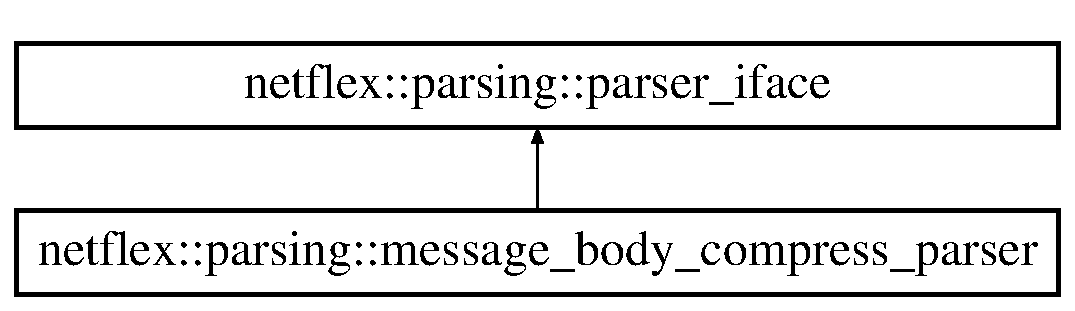
\includegraphics[height=2.000000cm]{classnetflex_1_1parsing_1_1message__body__compress__parser}
\end{center}
\end{figure}
\subsection*{Public Member Functions}
\begin{DoxyCompactItemize}
\item 
\mbox{\Hypertarget{classnetflex_1_1parsing_1_1message__body__compress__parser_a6cd3e2a01694e42f973640fa144e58e1}\label{classnetflex_1_1parsing_1_1message__body__compress__parser_a6cd3e2a01694e42f973640fa144e58e1}} 
\hyperlink{classnetflex_1_1parsing_1_1message__body__compress__parser_a6cd3e2a01694e42f973640fa144e58e1}{message\+\_\+body\+\_\+compress\+\_\+parser} (\hyperlink{classnetflex_1_1http_1_1request}{http\+::request} \&request)
\begin{DoxyCompactList}\small\item\em ctor \& dtor \end{DoxyCompactList}\item 
\mbox{\Hypertarget{classnetflex_1_1parsing_1_1message__body__compress__parser_a1d5e498f4b6ff6dfaaebc44a5548a429}\label{classnetflex_1_1parsing_1_1message__body__compress__parser_a1d5e498f4b6ff6dfaaebc44a5548a429}} 
\hyperlink{classnetflex_1_1parsing_1_1message__body__compress__parser_a1d5e498f4b6ff6dfaaebc44a5548a429}{message\+\_\+body\+\_\+compress\+\_\+parser} (const \hyperlink{classnetflex_1_1parsing_1_1message__body__compress__parser}{message\+\_\+body\+\_\+compress\+\_\+parser} \&)=delete
\begin{DoxyCompactList}\small\item\em copy ctor \& assignment operator \end{DoxyCompactList}\item 
\mbox{\Hypertarget{classnetflex_1_1parsing_1_1message__body__compress__parser_ab03ca2e5af5f21b934f020c661ad6ac1}\label{classnetflex_1_1parsing_1_1message__body__compress__parser_ab03ca2e5af5f21b934f020c661ad6ac1}} 
\hyperlink{classnetflex_1_1parsing_1_1message__body__compress__parser}{message\+\_\+body\+\_\+compress\+\_\+parser} \& {\bfseries operator=} (const \hyperlink{classnetflex_1_1parsing_1_1message__body__compress__parser}{message\+\_\+body\+\_\+compress\+\_\+parser} \&)=delete
\item 
\mbox{\Hypertarget{classnetflex_1_1parsing_1_1message__body__compress__parser_a75fc64c9be07c57fd44028862933387b}\label{classnetflex_1_1parsing_1_1message__body__compress__parser_a75fc64c9be07c57fd44028862933387b}} 
\hyperlink{classnetflex_1_1parsing_1_1parser__iface}{parser\+\_\+iface} \& \hyperlink{classnetflex_1_1parsing_1_1message__body__compress__parser_a75fc64c9be07c57fd44028862933387b}{operator$<$$<$} (std\+::string \&)
\begin{DoxyCompactList}\small\item\em \hyperlink{classnetflex_1_1parsing_1_1parser__iface}{parser\+\_\+iface} impl \end{DoxyCompactList}\item 
\mbox{\Hypertarget{classnetflex_1_1parsing_1_1message__body__compress__parser_ad963822a3d7ae17704fd7732925837f9}\label{classnetflex_1_1parsing_1_1message__body__compress__parser_ad963822a3d7ae17704fd7732925837f9}} 
bool \hyperlink{classnetflex_1_1parsing_1_1message__body__compress__parser_ad963822a3d7ae17704fd7732925837f9}{is\+\_\+done} (void) const
\begin{DoxyCompactList}\small\item\em returns whether the given http packet section has been fully parsed \end{DoxyCompactList}\end{DoxyCompactItemize}
\subsection*{Additional Inherited Members}


The documentation for this class was generated from the following file\+:\begin{DoxyCompactItemize}
\item 
includes/netflex/parsing/message\+\_\+body\+\_\+compress\+\_\+parser.\+hpp\end{DoxyCompactItemize}

\hypertarget{classnetflex_1_1parsing_1_1message__body__content__length__parser}{}\section{netflex\+:\+:parsing\+:\+:message\+\_\+body\+\_\+content\+\_\+length\+\_\+parser Class Reference}
\label{classnetflex_1_1parsing_1_1message__body__content__length__parser}\index{netflex\+::parsing\+::message\+\_\+body\+\_\+content\+\_\+length\+\_\+parser@{netflex\+::parsing\+::message\+\_\+body\+\_\+content\+\_\+length\+\_\+parser}}


{\ttfamily \#include $<$message\+\_\+body\+\_\+content\+\_\+length\+\_\+parser.\+hpp$>$}

Inheritance diagram for netflex\+:\+:parsing\+:\+:message\+\_\+body\+\_\+content\+\_\+length\+\_\+parser\+:\begin{figure}[H]
\begin{center}
\leavevmode
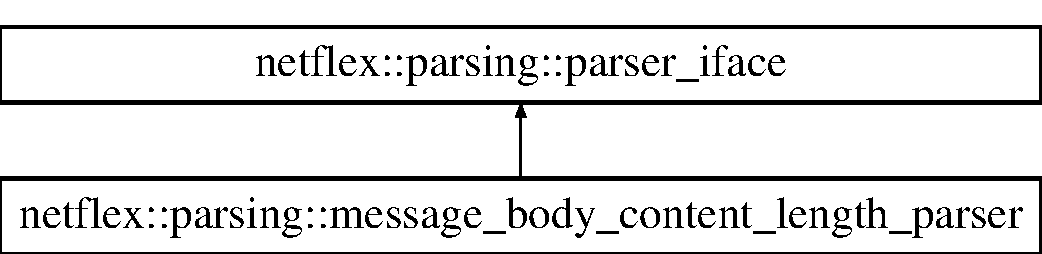
\includegraphics[height=2.000000cm]{classnetflex_1_1parsing_1_1message__body__content__length__parser}
\end{center}
\end{figure}
\subsection*{Public Member Functions}
\begin{DoxyCompactItemize}
\item 
\hyperlink{classnetflex_1_1parsing_1_1message__body__content__length__parser_a639fe3f1644ba35c46cdcb4de6973aee}{message\+\_\+body\+\_\+content\+\_\+length\+\_\+parser} (\hyperlink{classnetflex_1_1http_1_1request}{http\+::request} \&request)
\item 
\mbox{\Hypertarget{classnetflex_1_1parsing_1_1message__body__content__length__parser_abaa3ebcdf8b246c8a83e92de43cfa1fc}\label{classnetflex_1_1parsing_1_1message__body__content__length__parser_abaa3ebcdf8b246c8a83e92de43cfa1fc}} 
\hyperlink{classnetflex_1_1parsing_1_1message__body__content__length__parser_abaa3ebcdf8b246c8a83e92de43cfa1fc}{$\sim$message\+\_\+body\+\_\+content\+\_\+length\+\_\+parser} (void)=default
\begin{DoxyCompactList}\small\item\em default dtor \end{DoxyCompactList}\item 
\mbox{\Hypertarget{classnetflex_1_1parsing_1_1message__body__content__length__parser_ab273008d20c057036ea27c81e728f155}\label{classnetflex_1_1parsing_1_1message__body__content__length__parser_ab273008d20c057036ea27c81e728f155}} 
\hyperlink{classnetflex_1_1parsing_1_1message__body__content__length__parser_ab273008d20c057036ea27c81e728f155}{message\+\_\+body\+\_\+content\+\_\+length\+\_\+parser} (const \hyperlink{classnetflex_1_1parsing_1_1message__body__content__length__parser}{message\+\_\+body\+\_\+content\+\_\+length\+\_\+parser} \&)=delete
\begin{DoxyCompactList}\small\item\em copy ctor \end{DoxyCompactList}\item 
\mbox{\Hypertarget{classnetflex_1_1parsing_1_1message__body__content__length__parser_aa186661021a3432bfd349f34398cf5db}\label{classnetflex_1_1parsing_1_1message__body__content__length__parser_aa186661021a3432bfd349f34398cf5db}} 
\hyperlink{classnetflex_1_1parsing_1_1message__body__content__length__parser}{message\+\_\+body\+\_\+content\+\_\+length\+\_\+parser} \& \hyperlink{classnetflex_1_1parsing_1_1message__body__content__length__parser_aa186661021a3432bfd349f34398cf5db}{operator=} (const \hyperlink{classnetflex_1_1parsing_1_1message__body__content__length__parser}{message\+\_\+body\+\_\+content\+\_\+length\+\_\+parser} \&)=delete
\begin{DoxyCompactList}\small\item\em assignment operator \end{DoxyCompactList}\item 
\hyperlink{classnetflex_1_1parsing_1_1parser__iface}{parser\+\_\+iface} \& \hyperlink{classnetflex_1_1parsing_1_1message__body__content__length__parser_aedd5e9afda1868496de8c69c8ef0eae2}{operator$<$$<$} (std\+::string \&data)
\item 
bool \hyperlink{classnetflex_1_1parsing_1_1message__body__content__length__parser_abe03e2f2d6f61076cf147a4bcd7f80c5}{is\+\_\+done} (void) const
\end{DoxyCompactItemize}
\subsection*{Additional Inherited Members}


\subsection{Detailed Description}
parser for a Content-\/\+Length body 

\subsection{Constructor \& Destructor Documentation}
\mbox{\Hypertarget{classnetflex_1_1parsing_1_1message__body__content__length__parser_a639fe3f1644ba35c46cdcb4de6973aee}\label{classnetflex_1_1parsing_1_1message__body__content__length__parser_a639fe3f1644ba35c46cdcb4de6973aee}} 
\index{netflex\+::parsing\+::message\+\_\+body\+\_\+content\+\_\+length\+\_\+parser@{netflex\+::parsing\+::message\+\_\+body\+\_\+content\+\_\+length\+\_\+parser}!message\+\_\+body\+\_\+content\+\_\+length\+\_\+parser@{message\+\_\+body\+\_\+content\+\_\+length\+\_\+parser}}
\index{message\+\_\+body\+\_\+content\+\_\+length\+\_\+parser@{message\+\_\+body\+\_\+content\+\_\+length\+\_\+parser}!netflex\+::parsing\+::message\+\_\+body\+\_\+content\+\_\+length\+\_\+parser@{netflex\+::parsing\+::message\+\_\+body\+\_\+content\+\_\+length\+\_\+parser}}
\subsubsection{\texorpdfstring{message\+\_\+body\+\_\+content\+\_\+length\+\_\+parser()}{message\_body\_content\_length\_parser()}}
{\footnotesize\ttfamily netflex\+::parsing\+::message\+\_\+body\+\_\+content\+\_\+length\+\_\+parser\+::message\+\_\+body\+\_\+content\+\_\+length\+\_\+parser (\begin{DoxyParamCaption}\item[{\hyperlink{classnetflex_1_1http_1_1request}{http\+::request} \&}]{request }\end{DoxyParamCaption})\hspace{0.3cm}{\ttfamily [explicit]}}

default ctor


\begin{DoxyParams}{Parameters}
{\em request} & request to be initialized \\
\hline
\end{DoxyParams}


\subsection{Member Function Documentation}
\mbox{\Hypertarget{classnetflex_1_1parsing_1_1message__body__content__length__parser_abe03e2f2d6f61076cf147a4bcd7f80c5}\label{classnetflex_1_1parsing_1_1message__body__content__length__parser_abe03e2f2d6f61076cf147a4bcd7f80c5}} 
\index{netflex\+::parsing\+::message\+\_\+body\+\_\+content\+\_\+length\+\_\+parser@{netflex\+::parsing\+::message\+\_\+body\+\_\+content\+\_\+length\+\_\+parser}!is\+\_\+done@{is\+\_\+done}}
\index{is\+\_\+done@{is\+\_\+done}!netflex\+::parsing\+::message\+\_\+body\+\_\+content\+\_\+length\+\_\+parser@{netflex\+::parsing\+::message\+\_\+body\+\_\+content\+\_\+length\+\_\+parser}}
\subsubsection{\texorpdfstring{is\+\_\+done()}{is\_done()}}
{\footnotesize\ttfamily bool netflex\+::parsing\+::message\+\_\+body\+\_\+content\+\_\+length\+\_\+parser\+::is\+\_\+done (\begin{DoxyParamCaption}\item[{void}]{ }\end{DoxyParamCaption}) const\hspace{0.3cm}{\ttfamily [virtual]}}

\begin{DoxyReturn}{Returns}
whether the parsing is done or not 
\end{DoxyReturn}


Implements \hyperlink{classnetflex_1_1parsing_1_1parser__iface_afebd1cc50d5958f712dfac0c023fd162}{netflex\+::parsing\+::parser\+\_\+iface}.

\mbox{\Hypertarget{classnetflex_1_1parsing_1_1message__body__content__length__parser_aedd5e9afda1868496de8c69c8ef0eae2}\label{classnetflex_1_1parsing_1_1message__body__content__length__parser_aedd5e9afda1868496de8c69c8ef0eae2}} 
\index{netflex\+::parsing\+::message\+\_\+body\+\_\+content\+\_\+length\+\_\+parser@{netflex\+::parsing\+::message\+\_\+body\+\_\+content\+\_\+length\+\_\+parser}!operator$<$$<$@{operator$<$$<$}}
\index{operator$<$$<$@{operator$<$$<$}!netflex\+::parsing\+::message\+\_\+body\+\_\+content\+\_\+length\+\_\+parser@{netflex\+::parsing\+::message\+\_\+body\+\_\+content\+\_\+length\+\_\+parser}}
\subsubsection{\texorpdfstring{operator$<$$<$()}{operator<<()}}
{\footnotesize\ttfamily \hyperlink{classnetflex_1_1parsing_1_1parser__iface}{parser\+\_\+iface}\& netflex\+::parsing\+::message\+\_\+body\+\_\+content\+\_\+length\+\_\+parser\+::operator$<$$<$ (\begin{DoxyParamCaption}\item[{std\+::string \&}]{data }\end{DoxyParamCaption})\hspace{0.3cm}{\ttfamily [virtual]}}

consume input data to parse it and init the request if not enough data is passed in, this method would need to be called again later input data is modified whenever a token is consumed by parsing, even if parsing is incomplete or invalid invalid data would lead to a raised exception


\begin{DoxyParams}{Parameters}
{\em data} & input data to be parsed \\
\hline
\end{DoxyParams}
\begin{DoxyReturn}{Returns}
reference to the current object 
\end{DoxyReturn}


Implements \hyperlink{classnetflex_1_1parsing_1_1parser__iface_a6b092567e70a5c0bf7568e94d06f7154}{netflex\+::parsing\+::parser\+\_\+iface}.



The documentation for this class was generated from the following file\+:\begin{DoxyCompactItemize}
\item 
includes/netflex/parsing/message\+\_\+body\+\_\+content\+\_\+length\+\_\+parser.\+hpp\end{DoxyCompactItemize}

\hypertarget{classnetflex_1_1parsing_1_1message__body__deflate__parser}{}\section{netflex\+:\+:parsing\+:\+:message\+\_\+body\+\_\+deflate\+\_\+parser Class Reference}
\label{classnetflex_1_1parsing_1_1message__body__deflate__parser}\index{netflex\+::parsing\+::message\+\_\+body\+\_\+deflate\+\_\+parser@{netflex\+::parsing\+::message\+\_\+body\+\_\+deflate\+\_\+parser}}
Inheritance diagram for netflex\+:\+:parsing\+:\+:message\+\_\+body\+\_\+deflate\+\_\+parser\+:\begin{figure}[H]
\begin{center}
\leavevmode
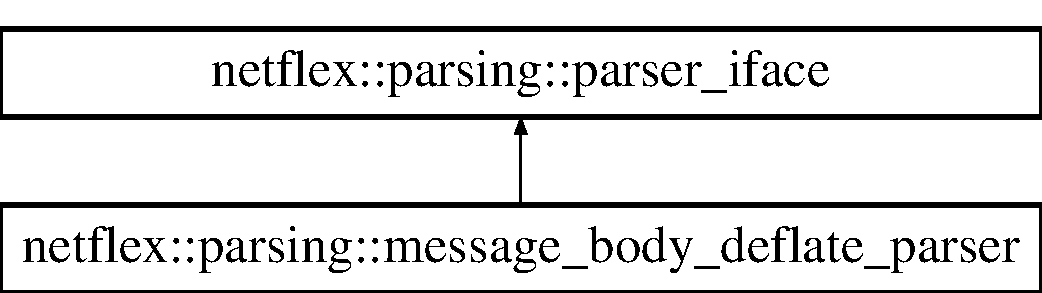
\includegraphics[height=2.000000cm]{classnetflex_1_1parsing_1_1message__body__deflate__parser}
\end{center}
\end{figure}
\subsection*{Public Member Functions}
\begin{DoxyCompactItemize}
\item 
\mbox{\Hypertarget{classnetflex_1_1parsing_1_1message__body__deflate__parser_a50f8b3c3bc5a6ad1b8bd63803d92c455}\label{classnetflex_1_1parsing_1_1message__body__deflate__parser_a50f8b3c3bc5a6ad1b8bd63803d92c455}} 
\hyperlink{classnetflex_1_1parsing_1_1message__body__deflate__parser_a50f8b3c3bc5a6ad1b8bd63803d92c455}{message\+\_\+body\+\_\+deflate\+\_\+parser} (\hyperlink{classnetflex_1_1http_1_1request}{http\+::request} \&request)
\begin{DoxyCompactList}\small\item\em ctor \& dtor \end{DoxyCompactList}\item 
\mbox{\Hypertarget{classnetflex_1_1parsing_1_1message__body__deflate__parser_a883c098ee9b13ef7c0986c1634794b0d}\label{classnetflex_1_1parsing_1_1message__body__deflate__parser_a883c098ee9b13ef7c0986c1634794b0d}} 
\hyperlink{classnetflex_1_1parsing_1_1message__body__deflate__parser_a883c098ee9b13ef7c0986c1634794b0d}{message\+\_\+body\+\_\+deflate\+\_\+parser} (const \hyperlink{classnetflex_1_1parsing_1_1message__body__deflate__parser}{message\+\_\+body\+\_\+deflate\+\_\+parser} \&)=delete
\begin{DoxyCompactList}\small\item\em copy ctor \& assignment operator \end{DoxyCompactList}\item 
\mbox{\Hypertarget{classnetflex_1_1parsing_1_1message__body__deflate__parser_a5d5b893c9f2e32b2ec09cf16ada13c36}\label{classnetflex_1_1parsing_1_1message__body__deflate__parser_a5d5b893c9f2e32b2ec09cf16ada13c36}} 
\hyperlink{classnetflex_1_1parsing_1_1message__body__deflate__parser}{message\+\_\+body\+\_\+deflate\+\_\+parser} \& {\bfseries operator=} (const \hyperlink{classnetflex_1_1parsing_1_1message__body__deflate__parser}{message\+\_\+body\+\_\+deflate\+\_\+parser} \&)=delete
\item 
\mbox{\Hypertarget{classnetflex_1_1parsing_1_1message__body__deflate__parser_af7ee85cc5edee4e1f6cf34bebccceaa4}\label{classnetflex_1_1parsing_1_1message__body__deflate__parser_af7ee85cc5edee4e1f6cf34bebccceaa4}} 
\hyperlink{classnetflex_1_1parsing_1_1parser__iface}{parser\+\_\+iface} \& \hyperlink{classnetflex_1_1parsing_1_1message__body__deflate__parser_af7ee85cc5edee4e1f6cf34bebccceaa4}{operator$<$$<$} (std\+::string \&)
\begin{DoxyCompactList}\small\item\em \hyperlink{classnetflex_1_1parsing_1_1parser__iface}{parser\+\_\+iface} impl \end{DoxyCompactList}\item 
\mbox{\Hypertarget{classnetflex_1_1parsing_1_1message__body__deflate__parser_a2e80b1cc5a930497653e200c72adc4e5}\label{classnetflex_1_1parsing_1_1message__body__deflate__parser_a2e80b1cc5a930497653e200c72adc4e5}} 
bool \hyperlink{classnetflex_1_1parsing_1_1message__body__deflate__parser_a2e80b1cc5a930497653e200c72adc4e5}{is\+\_\+done} (void) const
\begin{DoxyCompactList}\small\item\em returns whether the given http packet section has been fully parsed \end{DoxyCompactList}\end{DoxyCompactItemize}
\subsection*{Additional Inherited Members}


The documentation for this class was generated from the following file\+:\begin{DoxyCompactItemize}
\item 
includes/netflex/parsing/message\+\_\+body\+\_\+deflate\+\_\+parser.\+hpp\end{DoxyCompactItemize}

\hypertarget{classnetflex_1_1parsing_1_1message__body__gzip__parser}{}\section{netflex\+:\+:parsing\+:\+:message\+\_\+body\+\_\+gzip\+\_\+parser Class Reference}
\label{classnetflex_1_1parsing_1_1message__body__gzip__parser}\index{netflex\+::parsing\+::message\+\_\+body\+\_\+gzip\+\_\+parser@{netflex\+::parsing\+::message\+\_\+body\+\_\+gzip\+\_\+parser}}


{\ttfamily \#include $<$message\+\_\+body\+\_\+gzip\+\_\+parser.\+hpp$>$}

Inheritance diagram for netflex\+:\+:parsing\+:\+:message\+\_\+body\+\_\+gzip\+\_\+parser\+:\begin{figure}[H]
\begin{center}
\leavevmode
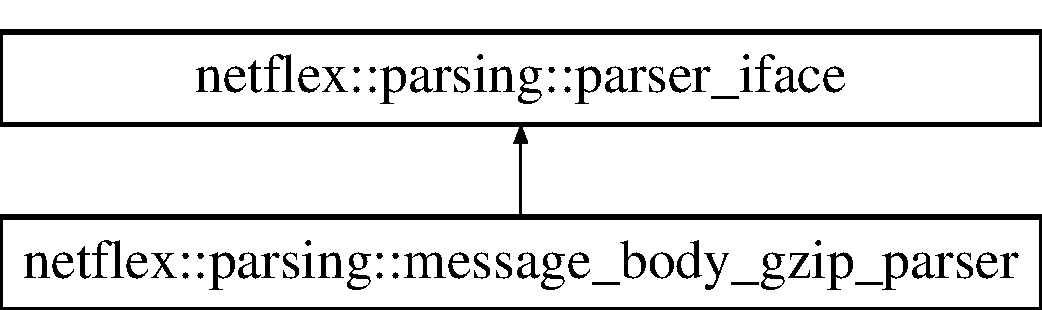
\includegraphics[height=2.000000cm]{classnetflex_1_1parsing_1_1message__body__gzip__parser}
\end{center}
\end{figure}
\subsection*{Public Member Functions}
\begin{DoxyCompactItemize}
\item 
\hyperlink{classnetflex_1_1parsing_1_1message__body__gzip__parser_a8f5b49b2af4bd6c96dad3959f04c763b}{message\+\_\+body\+\_\+gzip\+\_\+parser} (\hyperlink{classnetflex_1_1http_1_1request}{http\+::request} \&request)
\item 
\mbox{\Hypertarget{classnetflex_1_1parsing_1_1message__body__gzip__parser_a419851e77f95541063cfdaa9f0d65ecd}\label{classnetflex_1_1parsing_1_1message__body__gzip__parser_a419851e77f95541063cfdaa9f0d65ecd}} 
\hyperlink{classnetflex_1_1parsing_1_1message__body__gzip__parser_a419851e77f95541063cfdaa9f0d65ecd}{$\sim$message\+\_\+body\+\_\+gzip\+\_\+parser} (void)=default
\begin{DoxyCompactList}\small\item\em default dtor \end{DoxyCompactList}\item 
\mbox{\Hypertarget{classnetflex_1_1parsing_1_1message__body__gzip__parser_a5c516454893dbda1a8ff93d7815b12a9}\label{classnetflex_1_1parsing_1_1message__body__gzip__parser_a5c516454893dbda1a8ff93d7815b12a9}} 
\hyperlink{classnetflex_1_1parsing_1_1message__body__gzip__parser_a5c516454893dbda1a8ff93d7815b12a9}{message\+\_\+body\+\_\+gzip\+\_\+parser} (const \hyperlink{classnetflex_1_1parsing_1_1message__body__gzip__parser}{message\+\_\+body\+\_\+gzip\+\_\+parser} \&)=delete
\begin{DoxyCompactList}\small\item\em copy ctor \end{DoxyCompactList}\item 
\mbox{\Hypertarget{classnetflex_1_1parsing_1_1message__body__gzip__parser_ab28726f6d793f340cb630cfcaa6e3126}\label{classnetflex_1_1parsing_1_1message__body__gzip__parser_ab28726f6d793f340cb630cfcaa6e3126}} 
\hyperlink{classnetflex_1_1parsing_1_1message__body__gzip__parser}{message\+\_\+body\+\_\+gzip\+\_\+parser} \& \hyperlink{classnetflex_1_1parsing_1_1message__body__gzip__parser_ab28726f6d793f340cb630cfcaa6e3126}{operator=} (const \hyperlink{classnetflex_1_1parsing_1_1message__body__gzip__parser}{message\+\_\+body\+\_\+gzip\+\_\+parser} \&)=delete
\begin{DoxyCompactList}\small\item\em assignment operator \end{DoxyCompactList}\item 
\hyperlink{classnetflex_1_1parsing_1_1parser__iface}{parser\+\_\+iface} \& \hyperlink{classnetflex_1_1parsing_1_1message__body__gzip__parser_a5206f23709657035b665238966a5cf13}{operator$<$$<$} (std\+::string \&data)
\item 
bool \hyperlink{classnetflex_1_1parsing_1_1message__body__gzip__parser_a7751bc115acc99af5ab7d8f1a6de5581}{is\+\_\+done} (void) const
\end{DoxyCompactItemize}
\subsection*{Additional Inherited Members}


\subsection{Detailed Description}
parser for a gziped body 

\subsection{Constructor \& Destructor Documentation}
\mbox{\Hypertarget{classnetflex_1_1parsing_1_1message__body__gzip__parser_a8f5b49b2af4bd6c96dad3959f04c763b}\label{classnetflex_1_1parsing_1_1message__body__gzip__parser_a8f5b49b2af4bd6c96dad3959f04c763b}} 
\index{netflex\+::parsing\+::message\+\_\+body\+\_\+gzip\+\_\+parser@{netflex\+::parsing\+::message\+\_\+body\+\_\+gzip\+\_\+parser}!message\+\_\+body\+\_\+gzip\+\_\+parser@{message\+\_\+body\+\_\+gzip\+\_\+parser}}
\index{message\+\_\+body\+\_\+gzip\+\_\+parser@{message\+\_\+body\+\_\+gzip\+\_\+parser}!netflex\+::parsing\+::message\+\_\+body\+\_\+gzip\+\_\+parser@{netflex\+::parsing\+::message\+\_\+body\+\_\+gzip\+\_\+parser}}
\subsubsection{\texorpdfstring{message\+\_\+body\+\_\+gzip\+\_\+parser()}{message\_body\_gzip\_parser()}}
{\footnotesize\ttfamily netflex\+::parsing\+::message\+\_\+body\+\_\+gzip\+\_\+parser\+::message\+\_\+body\+\_\+gzip\+\_\+parser (\begin{DoxyParamCaption}\item[{\hyperlink{classnetflex_1_1http_1_1request}{http\+::request} \&}]{request }\end{DoxyParamCaption})\hspace{0.3cm}{\ttfamily [explicit]}}

default ctor


\begin{DoxyParams}{Parameters}
{\em request} & request to be initialized \\
\hline
\end{DoxyParams}


\subsection{Member Function Documentation}
\mbox{\Hypertarget{classnetflex_1_1parsing_1_1message__body__gzip__parser_a7751bc115acc99af5ab7d8f1a6de5581}\label{classnetflex_1_1parsing_1_1message__body__gzip__parser_a7751bc115acc99af5ab7d8f1a6de5581}} 
\index{netflex\+::parsing\+::message\+\_\+body\+\_\+gzip\+\_\+parser@{netflex\+::parsing\+::message\+\_\+body\+\_\+gzip\+\_\+parser}!is\+\_\+done@{is\+\_\+done}}
\index{is\+\_\+done@{is\+\_\+done}!netflex\+::parsing\+::message\+\_\+body\+\_\+gzip\+\_\+parser@{netflex\+::parsing\+::message\+\_\+body\+\_\+gzip\+\_\+parser}}
\subsubsection{\texorpdfstring{is\+\_\+done()}{is\_done()}}
{\footnotesize\ttfamily bool netflex\+::parsing\+::message\+\_\+body\+\_\+gzip\+\_\+parser\+::is\+\_\+done (\begin{DoxyParamCaption}\item[{void}]{ }\end{DoxyParamCaption}) const\hspace{0.3cm}{\ttfamily [virtual]}}

\begin{DoxyReturn}{Returns}
whether the parsing is done or not 
\end{DoxyReturn}


Implements \hyperlink{classnetflex_1_1parsing_1_1parser__iface_afebd1cc50d5958f712dfac0c023fd162}{netflex\+::parsing\+::parser\+\_\+iface}.

\mbox{\Hypertarget{classnetflex_1_1parsing_1_1message__body__gzip__parser_a5206f23709657035b665238966a5cf13}\label{classnetflex_1_1parsing_1_1message__body__gzip__parser_a5206f23709657035b665238966a5cf13}} 
\index{netflex\+::parsing\+::message\+\_\+body\+\_\+gzip\+\_\+parser@{netflex\+::parsing\+::message\+\_\+body\+\_\+gzip\+\_\+parser}!operator$<$$<$@{operator$<$$<$}}
\index{operator$<$$<$@{operator$<$$<$}!netflex\+::parsing\+::message\+\_\+body\+\_\+gzip\+\_\+parser@{netflex\+::parsing\+::message\+\_\+body\+\_\+gzip\+\_\+parser}}
\subsubsection{\texorpdfstring{operator$<$$<$()}{operator<<()}}
{\footnotesize\ttfamily \hyperlink{classnetflex_1_1parsing_1_1parser__iface}{parser\+\_\+iface}\& netflex\+::parsing\+::message\+\_\+body\+\_\+gzip\+\_\+parser\+::operator$<$$<$ (\begin{DoxyParamCaption}\item[{std\+::string \&}]{data }\end{DoxyParamCaption})\hspace{0.3cm}{\ttfamily [virtual]}}

consume input data to parse it and init the request if not enough data is passed in, this method would need to be called again later input data is modified whenever a token is consumed by parsing, even if parsing is incomplete or invalid invalid data would lead to a raised exception


\begin{DoxyParams}{Parameters}
{\em data} & input data to be parsed \\
\hline
\end{DoxyParams}
\begin{DoxyReturn}{Returns}
reference to the current object 
\end{DoxyReturn}


Implements \hyperlink{classnetflex_1_1parsing_1_1parser__iface_a6b092567e70a5c0bf7568e94d06f7154}{netflex\+::parsing\+::parser\+\_\+iface}.



The documentation for this class was generated from the following file\+:\begin{DoxyCompactItemize}
\item 
includes/netflex/parsing/message\+\_\+body\+\_\+gzip\+\_\+parser.\+hpp\end{DoxyCompactItemize}

\hypertarget{classnetflex_1_1parsing_1_1message__body__parser}{}\section{netflex\+:\+:parsing\+:\+:message\+\_\+body\+\_\+parser Class Reference}
\label{classnetflex_1_1parsing_1_1message__body__parser}\index{netflex\+::parsing\+::message\+\_\+body\+\_\+parser@{netflex\+::parsing\+::message\+\_\+body\+\_\+parser}}


{\ttfamily \#include $<$message\+\_\+body\+\_\+parser.\+hpp$>$}

Inheritance diagram for netflex\+:\+:parsing\+:\+:message\+\_\+body\+\_\+parser\+:\begin{figure}[H]
\begin{center}
\leavevmode
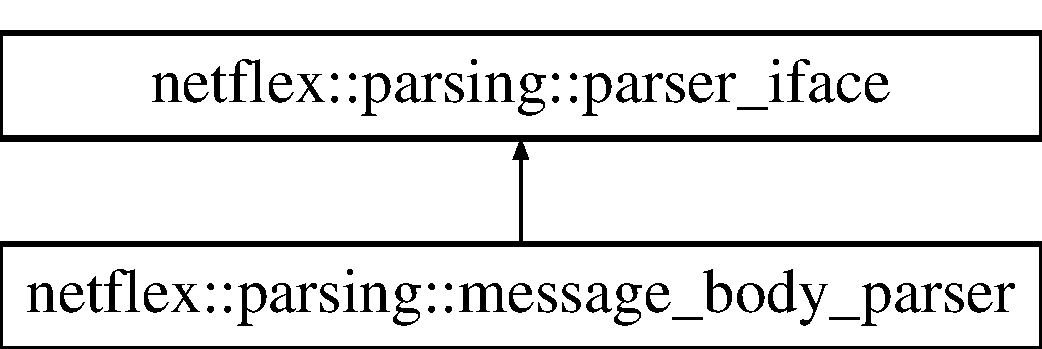
\includegraphics[height=2.000000cm]{classnetflex_1_1parsing_1_1message__body__parser}
\end{center}
\end{figure}
\subsection*{Public Member Functions}
\begin{DoxyCompactItemize}
\item 
\hyperlink{classnetflex_1_1parsing_1_1message__body__parser_a04a55d3b4b1dcfac47fd21fe2606da5f}{message\+\_\+body\+\_\+parser} (\hyperlink{classnetflex_1_1http_1_1request}{http\+::request} \&request)
\item 
\mbox{\Hypertarget{classnetflex_1_1parsing_1_1message__body__parser_a301f2b57282242ae37c0d094c5ad6951}\label{classnetflex_1_1parsing_1_1message__body__parser_a301f2b57282242ae37c0d094c5ad6951}} 
\hyperlink{classnetflex_1_1parsing_1_1message__body__parser_a301f2b57282242ae37c0d094c5ad6951}{$\sim$message\+\_\+body\+\_\+parser} (void)=default
\begin{DoxyCompactList}\small\item\em default dtor \end{DoxyCompactList}\item 
\mbox{\Hypertarget{classnetflex_1_1parsing_1_1message__body__parser_a0ef5ba4567c214272bf7ff84a98b5447}\label{classnetflex_1_1parsing_1_1message__body__parser_a0ef5ba4567c214272bf7ff84a98b5447}} 
\hyperlink{classnetflex_1_1parsing_1_1message__body__parser_a0ef5ba4567c214272bf7ff84a98b5447}{message\+\_\+body\+\_\+parser} (const \hyperlink{classnetflex_1_1parsing_1_1message__body__parser}{message\+\_\+body\+\_\+parser} \&)=delete
\begin{DoxyCompactList}\small\item\em copy ctor \end{DoxyCompactList}\item 
\mbox{\Hypertarget{classnetflex_1_1parsing_1_1message__body__parser_a0c5708195cecc7688ec3260ed38c5f88}\label{classnetflex_1_1parsing_1_1message__body__parser_a0c5708195cecc7688ec3260ed38c5f88}} 
\hyperlink{classnetflex_1_1parsing_1_1message__body__parser}{message\+\_\+body\+\_\+parser} \& \hyperlink{classnetflex_1_1parsing_1_1message__body__parser_a0c5708195cecc7688ec3260ed38c5f88}{operator=} (const \hyperlink{classnetflex_1_1parsing_1_1message__body__parser}{message\+\_\+body\+\_\+parser} \&)=delete
\begin{DoxyCompactList}\small\item\em assignment operator \end{DoxyCompactList}\item 
\hyperlink{classnetflex_1_1parsing_1_1parser__iface}{parser\+\_\+iface} \& \hyperlink{classnetflex_1_1parsing_1_1message__body__parser_a891c157d04d1fc59c1524672c4574570}{operator$<$$<$} (std\+::string \&data)
\item 
bool \hyperlink{classnetflex_1_1parsing_1_1message__body__parser_a71557821eaea2a6b629f86165fbc2f52}{is\+\_\+done} (void) const
\end{DoxyCompactItemize}
\subsection*{Additional Inherited Members}


\subsection{Detailed Description}
parser for body 

\subsection{Constructor \& Destructor Documentation}
\mbox{\Hypertarget{classnetflex_1_1parsing_1_1message__body__parser_a04a55d3b4b1dcfac47fd21fe2606da5f}\label{classnetflex_1_1parsing_1_1message__body__parser_a04a55d3b4b1dcfac47fd21fe2606da5f}} 
\index{netflex\+::parsing\+::message\+\_\+body\+\_\+parser@{netflex\+::parsing\+::message\+\_\+body\+\_\+parser}!message\+\_\+body\+\_\+parser@{message\+\_\+body\+\_\+parser}}
\index{message\+\_\+body\+\_\+parser@{message\+\_\+body\+\_\+parser}!netflex\+::parsing\+::message\+\_\+body\+\_\+parser@{netflex\+::parsing\+::message\+\_\+body\+\_\+parser}}
\subsubsection{\texorpdfstring{message\+\_\+body\+\_\+parser()}{message\_body\_parser()}}
{\footnotesize\ttfamily netflex\+::parsing\+::message\+\_\+body\+\_\+parser\+::message\+\_\+body\+\_\+parser (\begin{DoxyParamCaption}\item[{\hyperlink{classnetflex_1_1http_1_1request}{http\+::request} \&}]{request }\end{DoxyParamCaption})\hspace{0.3cm}{\ttfamily [explicit]}}

default ctor


\begin{DoxyParams}{Parameters}
{\em request} & request to be initialized \\
\hline
\end{DoxyParams}


\subsection{Member Function Documentation}
\mbox{\Hypertarget{classnetflex_1_1parsing_1_1message__body__parser_a71557821eaea2a6b629f86165fbc2f52}\label{classnetflex_1_1parsing_1_1message__body__parser_a71557821eaea2a6b629f86165fbc2f52}} 
\index{netflex\+::parsing\+::message\+\_\+body\+\_\+parser@{netflex\+::parsing\+::message\+\_\+body\+\_\+parser}!is\+\_\+done@{is\+\_\+done}}
\index{is\+\_\+done@{is\+\_\+done}!netflex\+::parsing\+::message\+\_\+body\+\_\+parser@{netflex\+::parsing\+::message\+\_\+body\+\_\+parser}}
\subsubsection{\texorpdfstring{is\+\_\+done()}{is\_done()}}
{\footnotesize\ttfamily bool netflex\+::parsing\+::message\+\_\+body\+\_\+parser\+::is\+\_\+done (\begin{DoxyParamCaption}\item[{void}]{ }\end{DoxyParamCaption}) const\hspace{0.3cm}{\ttfamily [virtual]}}

\begin{DoxyReturn}{Returns}
whether the parsing is done or not 
\end{DoxyReturn}


Implements \hyperlink{classnetflex_1_1parsing_1_1parser__iface_afebd1cc50d5958f712dfac0c023fd162}{netflex\+::parsing\+::parser\+\_\+iface}.

\mbox{\Hypertarget{classnetflex_1_1parsing_1_1message__body__parser_a891c157d04d1fc59c1524672c4574570}\label{classnetflex_1_1parsing_1_1message__body__parser_a891c157d04d1fc59c1524672c4574570}} 
\index{netflex\+::parsing\+::message\+\_\+body\+\_\+parser@{netflex\+::parsing\+::message\+\_\+body\+\_\+parser}!operator$<$$<$@{operator$<$$<$}}
\index{operator$<$$<$@{operator$<$$<$}!netflex\+::parsing\+::message\+\_\+body\+\_\+parser@{netflex\+::parsing\+::message\+\_\+body\+\_\+parser}}
\subsubsection{\texorpdfstring{operator$<$$<$()}{operator<<()}}
{\footnotesize\ttfamily \hyperlink{classnetflex_1_1parsing_1_1parser__iface}{parser\+\_\+iface}\& netflex\+::parsing\+::message\+\_\+body\+\_\+parser\+::operator$<$$<$ (\begin{DoxyParamCaption}\item[{std\+::string \&}]{data }\end{DoxyParamCaption})\hspace{0.3cm}{\ttfamily [virtual]}}

consume input data to parse it and init the request if not enough data is passed in, this method would need to be called again later input data is modified whenever a token is consumed by parsing, even if parsing is incomplete or invalid invalid data would lead to a raised exception


\begin{DoxyParams}{Parameters}
{\em data} & input data to be parsed \\
\hline
\end{DoxyParams}
\begin{DoxyReturn}{Returns}
reference to the current object 
\end{DoxyReturn}


Implements \hyperlink{classnetflex_1_1parsing_1_1parser__iface_a6b092567e70a5c0bf7568e94d06f7154}{netflex\+::parsing\+::parser\+\_\+iface}.



The documentation for this class was generated from the following file\+:\begin{DoxyCompactItemize}
\item 
includes/netflex/parsing/message\+\_\+body\+\_\+parser.\+hpp\end{DoxyCompactItemize}

\hypertarget{classnetflex_1_1routing_1_1middleware__chain}{}\section{netflex\+:\+:routing\+:\+:middleware\+\_\+chain Class Reference}
\label{classnetflex_1_1routing_1_1middleware__chain}\index{netflex\+::routing\+::middleware\+\_\+chain@{netflex\+::routing\+::middleware\+\_\+chain}}


{\ttfamily \#include $<$middleware\+\_\+chain.\+hpp$>$}

\subsection*{Public Member Functions}
\begin{DoxyCompactItemize}
\item 
\hyperlink{classnetflex_1_1routing_1_1middleware__chain_a1ca46e620562de94f0f18bda55d5dc6b}{middleware\+\_\+chain} (const std\+::list$<$ middleware\+\_\+t $>$ \&middlewares, \hyperlink{classnetflex_1_1http_1_1request}{http\+::request} \&request, \hyperlink{classnetflex_1_1http_1_1response}{http\+::response} \&response)
\item 
\mbox{\Hypertarget{classnetflex_1_1routing_1_1middleware__chain_a146dc01f9446f08f5e82d5c45fce9ca5}\label{classnetflex_1_1routing_1_1middleware__chain_a146dc01f9446f08f5e82d5c45fce9ca5}} 
\hyperlink{classnetflex_1_1routing_1_1middleware__chain_a146dc01f9446f08f5e82d5c45fce9ca5}{$\sim$middleware\+\_\+chain} (void)=default
\begin{DoxyCompactList}\small\item\em default dtor \end{DoxyCompactList}\item 
\mbox{\Hypertarget{classnetflex_1_1routing_1_1middleware__chain_ae9735fec43573278a01312692c5aff55}\label{classnetflex_1_1routing_1_1middleware__chain_ae9735fec43573278a01312692c5aff55}} 
\hyperlink{classnetflex_1_1routing_1_1middleware__chain_ae9735fec43573278a01312692c5aff55}{middleware\+\_\+chain} (const \hyperlink{classnetflex_1_1routing_1_1middleware__chain}{middleware\+\_\+chain} \&)=default
\begin{DoxyCompactList}\small\item\em copy ctor \end{DoxyCompactList}\item 
\mbox{\Hypertarget{classnetflex_1_1routing_1_1middleware__chain_a292af104bd22249848832886cdd40587}\label{classnetflex_1_1routing_1_1middleware__chain_a292af104bd22249848832886cdd40587}} 
\hyperlink{classnetflex_1_1routing_1_1middleware__chain}{middleware\+\_\+chain} \& \hyperlink{classnetflex_1_1routing_1_1middleware__chain_a292af104bd22249848832886cdd40587}{operator=} (const \hyperlink{classnetflex_1_1routing_1_1middleware__chain}{middleware\+\_\+chain} \&)=default
\begin{DoxyCompactList}\small\item\em assignment operator \end{DoxyCompactList}\item 
void \hyperlink{classnetflex_1_1routing_1_1middleware__chain_a762a6cce9e788dd6bb3261336d4bb841}{proceed} (void)
\end{DoxyCompactItemize}


\subsection{Detailed Description}
contains a chain of middlewares to execute used to manage execution of middlewares in the right order (and possibly stop the execution if necessary) 

\subsection{Constructor \& Destructor Documentation}
\mbox{\Hypertarget{classnetflex_1_1routing_1_1middleware__chain_a1ca46e620562de94f0f18bda55d5dc6b}\label{classnetflex_1_1routing_1_1middleware__chain_a1ca46e620562de94f0f18bda55d5dc6b}} 
\index{netflex\+::routing\+::middleware\+\_\+chain@{netflex\+::routing\+::middleware\+\_\+chain}!middleware\+\_\+chain@{middleware\+\_\+chain}}
\index{middleware\+\_\+chain@{middleware\+\_\+chain}!netflex\+::routing\+::middleware\+\_\+chain@{netflex\+::routing\+::middleware\+\_\+chain}}
\subsubsection{\texorpdfstring{middleware\+\_\+chain()}{middleware\_chain()}}
{\footnotesize\ttfamily netflex\+::routing\+::middleware\+\_\+chain\+::middleware\+\_\+chain (\begin{DoxyParamCaption}\item[{const std\+::list$<$ middleware\+\_\+t $>$ \&}]{middlewares,  }\item[{\hyperlink{classnetflex_1_1http_1_1request}{http\+::request} \&}]{request,  }\item[{\hyperlink{classnetflex_1_1http_1_1response}{http\+::response} \&}]{response }\end{DoxyParamCaption})}

ctor


\begin{DoxyParams}{Parameters}
{\em middlewares} & middlewares to be managed by the middleware chain. middleware should be ordered from lowest level (first executed) to highest level (last to be executed) \\
\hline
{\em request} & request to be passed as parameter to each middleware \\
\hline
{\em response} & response to be passed as parameter to each middleware \\
\hline
\end{DoxyParams}


\subsection{Member Function Documentation}
\mbox{\Hypertarget{classnetflex_1_1routing_1_1middleware__chain_a762a6cce9e788dd6bb3261336d4bb841}\label{classnetflex_1_1routing_1_1middleware__chain_a762a6cce9e788dd6bb3261336d4bb841}} 
\index{netflex\+::routing\+::middleware\+\_\+chain@{netflex\+::routing\+::middleware\+\_\+chain}!proceed@{proceed}}
\index{proceed@{proceed}!netflex\+::routing\+::middleware\+\_\+chain@{netflex\+::routing\+::middleware\+\_\+chain}}
\subsubsection{\texorpdfstring{proceed()}{proceed()}}
{\footnotesize\ttfamily void netflex\+::routing\+::middleware\+\_\+chain\+::proceed (\begin{DoxyParamCaption}\item[{void}]{ }\end{DoxyParamCaption})}

proceed to next middleware to be executed or return if nothing needs to be executed anymore 

The documentation for this class was generated from the following file\+:\begin{DoxyCompactItemize}
\item 
includes/netflex/routing/middleware\+\_\+chain.\+hpp\end{DoxyCompactItemize}

\hypertarget{classnetflex_1_1netflex__error}{}\section{netflex\+:\+:netflex\+\_\+error Class Reference}
\label{classnetflex_1_1netflex__error}\index{netflex\+::netflex\+\_\+error@{netflex\+::netflex\+\_\+error}}
Inheritance diagram for netflex\+:\+:netflex\+\_\+error\+:\begin{figure}[H]
\begin{center}
\leavevmode
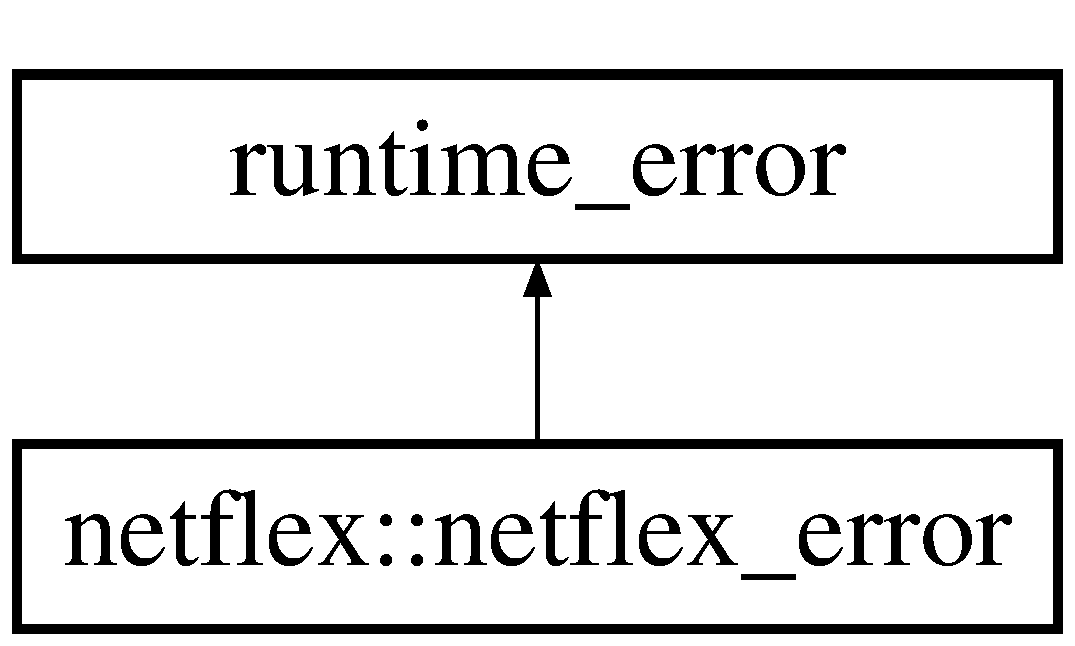
\includegraphics[height=2.000000cm]{classnetflex_1_1netflex__error}
\end{center}
\end{figure}
\subsection*{Public Member Functions}
\begin{DoxyCompactItemize}
\item 
\mbox{\Hypertarget{classnetflex_1_1netflex__error_ac7410912ae60826d4d3c517bc77bd53d}\label{classnetflex_1_1netflex__error_ac7410912ae60826d4d3c517bc77bd53d}} 
{\bfseries netflex\+\_\+error} (const std\+::string \&msg)
\item 
\mbox{\Hypertarget{classnetflex_1_1netflex__error_a1b16bd2445517eed5b9e0e276e73a023}\label{classnetflex_1_1netflex__error_a1b16bd2445517eed5b9e0e276e73a023}} 
{\bfseries netflex\+\_\+error} (const char $\ast$msg)
\end{DoxyCompactItemize}


The documentation for this class was generated from the following file\+:\begin{DoxyCompactItemize}
\item 
includes/netflex/misc/error.\+hpp\end{DoxyCompactItemize}

\hypertarget{classnetflex_1_1parsing_1_1parser__iface}{}\section{netflex\+:\+:parsing\+:\+:parser\+\_\+iface Class Reference}
\label{classnetflex_1_1parsing_1_1parser__iface}\index{netflex\+::parsing\+::parser\+\_\+iface@{netflex\+::parsing\+::parser\+\_\+iface}}
Inheritance diagram for netflex\+:\+:parsing\+:\+:parser\+\_\+iface\+:\begin{figure}[H]
\begin{center}
\leavevmode
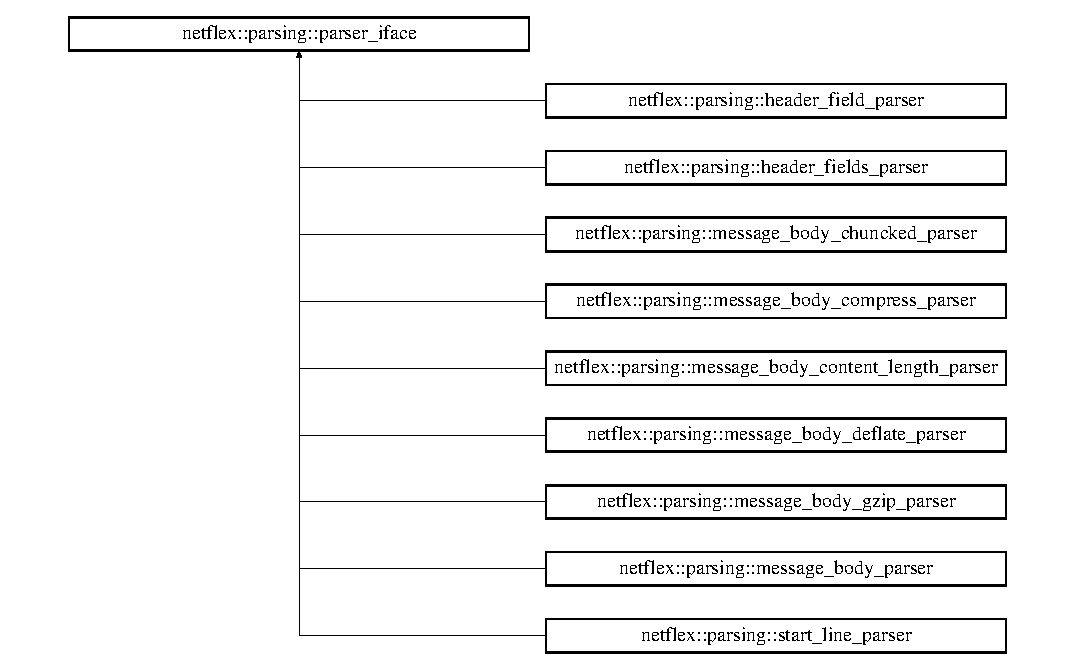
\includegraphics[height=8.536586cm]{classnetflex_1_1parsing_1_1parser__iface}
\end{center}
\end{figure}
\subsection*{Public Member Functions}
\begin{DoxyCompactItemize}
\item 
\mbox{\Hypertarget{classnetflex_1_1parsing_1_1parser__iface_aacba4e88059a0802b22c19b324bae9ec}\label{classnetflex_1_1parsing_1_1parser__iface_aacba4e88059a0802b22c19b324bae9ec}} 
\hyperlink{classnetflex_1_1parsing_1_1parser__iface_aacba4e88059a0802b22c19b324bae9ec}{parser\+\_\+iface} (\hyperlink{classnetflex_1_1http_1_1request}{http\+::request} \&)
\begin{DoxyCompactList}\small\item\em ctor \& virtual dtor \end{DoxyCompactList}\item 
virtual \hyperlink{classnetflex_1_1parsing_1_1parser__iface}{parser\+\_\+iface} \& \hyperlink{classnetflex_1_1parsing_1_1parser__iface_ae41c581b5cb219fed4cf5fccf27011c3}{operator$<$$<$} (std\+::string \&)=0
\item 
\mbox{\Hypertarget{classnetflex_1_1parsing_1_1parser__iface_afebd1cc50d5958f712dfac0c023fd162}\label{classnetflex_1_1parsing_1_1parser__iface_afebd1cc50d5958f712dfac0c023fd162}} 
virtual bool \hyperlink{classnetflex_1_1parsing_1_1parser__iface_afebd1cc50d5958f712dfac0c023fd162}{is\+\_\+done} (void) const =0
\begin{DoxyCompactList}\small\item\em returns whether the given http packet section has been fully parsed \end{DoxyCompactList}\end{DoxyCompactItemize}
\subsection*{Protected Attributes}
\begin{DoxyCompactItemize}
\item 
\mbox{\Hypertarget{classnetflex_1_1parsing_1_1parser__iface_a893c1abb768c2884318d7f35d315621b}\label{classnetflex_1_1parsing_1_1parser__iface_a893c1abb768c2884318d7f35d315621b}} 
\hyperlink{classnetflex_1_1http_1_1request}{http\+::request} \& \hyperlink{classnetflex_1_1parsing_1_1parser__iface_a893c1abb768c2884318d7f35d315621b}{m\+\_\+request}
\begin{DoxyCompactList}\small\item\em request \end{DoxyCompactList}\end{DoxyCompactItemize}


\subsection{Member Function Documentation}
\mbox{\Hypertarget{classnetflex_1_1parsing_1_1parser__iface_ae41c581b5cb219fed4cf5fccf27011c3}\label{classnetflex_1_1parsing_1_1parser__iface_ae41c581b5cb219fed4cf5fccf27011c3}} 
\index{netflex\+::parsing\+::parser\+\_\+iface@{netflex\+::parsing\+::parser\+\_\+iface}!operator$<$$<$@{operator$<$$<$}}
\index{operator$<$$<$@{operator$<$$<$}!netflex\+::parsing\+::parser\+\_\+iface@{netflex\+::parsing\+::parser\+\_\+iface}}
\subsubsection{\texorpdfstring{operator$<$$<$()}{operator<<()}}
{\footnotesize\ttfamily virtual \hyperlink{classnetflex_1_1parsing_1_1parser__iface}{parser\+\_\+iface}\& netflex\+::parsing\+::parser\+\_\+iface\+::operator$<$$<$ (\begin{DoxyParamCaption}\item[{std\+::string \&}]{ }\end{DoxyParamCaption})\hspace{0.3cm}{\ttfamily [pure virtual]}}

take data as parameter which is consumed to build the reply every bytes used to build the reply must be removed from the buffer passed as parameter in case of invalid format, an \hyperlink{classnetflex_1_1netflex__error}{netflex\+\_\+error} exception will be raised 

Implemented in \hyperlink{classnetflex_1_1parsing_1_1header__fields__parser_a255c485598692bee975e6db49d8ec13c}{netflex\+::parsing\+::header\+\_\+fields\+\_\+parser}, \hyperlink{classnetflex_1_1parsing_1_1start__line__parser_a663858012ee38e99d0c39444221bf4b5}{netflex\+::parsing\+::start\+\_\+line\+\_\+parser}, \hyperlink{classnetflex_1_1parsing_1_1header__field__parser_acdb399c2199106c99a2fcb4db1fbebca}{netflex\+::parsing\+::header\+\_\+field\+\_\+parser}, \hyperlink{classnetflex_1_1parsing_1_1message__body__parser_adb35dd992073f27e5c85d13453cd3db6}{netflex\+::parsing\+::message\+\_\+body\+\_\+parser}, \hyperlink{classnetflex_1_1parsing_1_1message__body__content__length__parser_a57265653361c2c29919799e2a7346a48}{netflex\+::parsing\+::message\+\_\+body\+\_\+content\+\_\+length\+\_\+parser}, \hyperlink{classnetflex_1_1parsing_1_1message__body__chuncked__parser_ac7a1529423ff3e606f418a6c5853e47d}{netflex\+::parsing\+::message\+\_\+body\+\_\+chuncked\+\_\+parser}, \hyperlink{classnetflex_1_1parsing_1_1message__body__compress__parser_a75fc64c9be07c57fd44028862933387b}{netflex\+::parsing\+::message\+\_\+body\+\_\+compress\+\_\+parser}, \hyperlink{classnetflex_1_1parsing_1_1message__body__deflate__parser_af7ee85cc5edee4e1f6cf34bebccceaa4}{netflex\+::parsing\+::message\+\_\+body\+\_\+deflate\+\_\+parser}, and \hyperlink{classnetflex_1_1parsing_1_1message__body__gzip__parser_a5adc84970912dcd766bb559dff7fe582}{netflex\+::parsing\+::message\+\_\+body\+\_\+gzip\+\_\+parser}.



The documentation for this class was generated from the following file\+:\begin{DoxyCompactItemize}
\item 
includes/netflex/parsing/parser\+\_\+iface.\+hpp\end{DoxyCompactItemize}

\hypertarget{classnetflex_1_1http_1_1request}{}\section{netflex\+:\+:http\+:\+:request Class Reference}
\label{classnetflex_1_1http_1_1request}\index{netflex\+::http\+::request@{netflex\+::http\+::request}}
\subsection*{Public Member Functions}
\begin{DoxyCompactItemize}
\item 
\mbox{\Hypertarget{classnetflex_1_1http_1_1request_a1c2202c8142807f69cd4bb627af2a3d2}\label{classnetflex_1_1http_1_1request_a1c2202c8142807f69cd4bb627af2a3d2}} 
\hyperlink{classnetflex_1_1http_1_1request_a1c2202c8142807f69cd4bb627af2a3d2}{request} (void)=default
\begin{DoxyCompactList}\small\item\em ctor \& dtor \end{DoxyCompactList}\item 
\mbox{\Hypertarget{classnetflex_1_1http_1_1request_af184b288745bda0dc34aec705ec5807e}\label{classnetflex_1_1http_1_1request_af184b288745bda0dc34aec705ec5807e}} 
\hyperlink{classnetflex_1_1http_1_1request_af184b288745bda0dc34aec705ec5807e}{request} (const \hyperlink{classnetflex_1_1http_1_1request}{request} \&)=default
\begin{DoxyCompactList}\small\item\em copy ctor \& assignment operator \end{DoxyCompactList}\item 
\mbox{\Hypertarget{classnetflex_1_1http_1_1request_aef5f7d7812a7fb94f85715fcdcf3686f}\label{classnetflex_1_1http_1_1request_aef5f7d7812a7fb94f85715fcdcf3686f}} 
\hyperlink{classnetflex_1_1http_1_1request}{request} \& {\bfseries operator=} (const \hyperlink{classnetflex_1_1http_1_1request}{request} \&)=default
\item 
\mbox{\Hypertarget{classnetflex_1_1http_1_1request_a465930c432dc303f6767858e971eda56}\label{classnetflex_1_1http_1_1request_a465930c432dc303f6767858e971eda56}} 
method \hyperlink{classnetflex_1_1http_1_1request_a465930c432dc303f6767858e971eda56}{get\+\_\+method} (void) const
\begin{DoxyCompactList}\small\item\em start line information \end{DoxyCompactList}\item 
\mbox{\Hypertarget{classnetflex_1_1http_1_1request_a708887a8c3a3582dbec9e1e5e2ec7b0b}\label{classnetflex_1_1http_1_1request_a708887a8c3a3582dbec9e1e5e2ec7b0b}} 
const std\+::string \& {\bfseries get\+\_\+raw\+\_\+method} (void) const
\item 
\mbox{\Hypertarget{classnetflex_1_1http_1_1request_aed90cb36a29b9bd2b0346ba0f399615a}\label{classnetflex_1_1http_1_1request_aed90cb36a29b9bd2b0346ba0f399615a}} 
const std\+::string \& {\bfseries get\+\_\+target} (void) const
\item 
\mbox{\Hypertarget{classnetflex_1_1http_1_1request_ab0cabbb537eb7470d06f4c8039d0e7cb}\label{classnetflex_1_1http_1_1request_ab0cabbb537eb7470d06f4c8039d0e7cb}} 
const std\+::string \& {\bfseries get\+\_\+http\+\_\+version} (void) const
\item 
\mbox{\Hypertarget{classnetflex_1_1http_1_1request_a7210ff25735da523403171152ff653d4}\label{classnetflex_1_1http_1_1request_a7210ff25735da523403171152ff653d4}} 
void {\bfseries set\+\_\+method} (method method)
\item 
\mbox{\Hypertarget{classnetflex_1_1http_1_1request_ad7e544191ac0fc2b97460265bccb4353}\label{classnetflex_1_1http_1_1request_ad7e544191ac0fc2b97460265bccb4353}} 
void {\bfseries set\+\_\+raw\+\_\+method} (const std\+::string \&method)
\item 
\mbox{\Hypertarget{classnetflex_1_1http_1_1request_ab8d678abf27538c7b3d7aade35496b06}\label{classnetflex_1_1http_1_1request_ab8d678abf27538c7b3d7aade35496b06}} 
void {\bfseries set\+\_\+target} (const std\+::string \&target)
\item 
\mbox{\Hypertarget{classnetflex_1_1http_1_1request_ab2c0c3caea31016028defd3b76035bd3}\label{classnetflex_1_1http_1_1request_ab2c0c3caea31016028defd3b76035bd3}} 
void {\bfseries set\+\_\+http\+\_\+version} (const std\+::string \&http\+\_\+version)
\item 
\mbox{\Hypertarget{classnetflex_1_1http_1_1request_a5d94ca7f1b6ce44a27c655570f2b8899}\label{classnetflex_1_1http_1_1request_a5d94ca7f1b6ce44a27c655570f2b8899}} 
const std\+::string \& \hyperlink{classnetflex_1_1http_1_1request_a5d94ca7f1b6ce44a27c655570f2b8899}{get\+\_\+header} (const std\+::string \&name) const
\begin{DoxyCompactList}\small\item\em headers information \end{DoxyCompactList}\item 
\mbox{\Hypertarget{classnetflex_1_1http_1_1request_a20a9b71acd61945261bbeaf81a73caf8}\label{classnetflex_1_1http_1_1request_a20a9b71acd61945261bbeaf81a73caf8}} 
const header\+\_\+list\+\_\+t \& {\bfseries get\+\_\+headers} (void) const
\item 
\mbox{\Hypertarget{classnetflex_1_1http_1_1request_aacda09c64841cb272c08262b6bae68a8}\label{classnetflex_1_1http_1_1request_aacda09c64841cb272c08262b6bae68a8}} 
void {\bfseries set\+\_\+headers} (const header\+\_\+list\+\_\+t \&headers)
\item 
\mbox{\Hypertarget{classnetflex_1_1http_1_1request_a18b1513d2b6a274cae832ad13dbe7760}\label{classnetflex_1_1http_1_1request_a18b1513d2b6a274cae832ad13dbe7760}} 
void {\bfseries add\+\_\+header} (const \hyperlink{structnetflex_1_1http_1_1header}{header} \&\hyperlink{structnetflex_1_1http_1_1header}{header})
\item 
\mbox{\Hypertarget{classnetflex_1_1http_1_1request_a906fb3043367133866daa9f18ad97393}\label{classnetflex_1_1http_1_1request_a906fb3043367133866daa9f18ad97393}} 
bool {\bfseries has\+\_\+header} (const std\+::string \&name) const
\item 
\mbox{\Hypertarget{classnetflex_1_1http_1_1request_ab598096641d91c5dc961e153cf47e445}\label{classnetflex_1_1http_1_1request_ab598096641d91c5dc961e153cf47e445}} 
void {\bfseries remove\+\_\+header} (const std\+::string \&name)
\item 
\mbox{\Hypertarget{classnetflex_1_1http_1_1request_a15483d8fc6a9af72832cb38b12457edf}\label{classnetflex_1_1http_1_1request_a15483d8fc6a9af72832cb38b12457edf}} 
const std\+::string \& \hyperlink{classnetflex_1_1http_1_1request_a15483d8fc6a9af72832cb38b12457edf}{get\+\_\+path} (void) const
\begin{DoxyCompactList}\small\item\em path \& params \end{DoxyCompactList}\item 
\mbox{\Hypertarget{classnetflex_1_1http_1_1request_a3c1cf98cae207060ee3f456a5bda0335}\label{classnetflex_1_1http_1_1request_a3c1cf98cae207060ee3f456a5bda0335}} 
const routing\+::params\+\_\+t \& {\bfseries get\+\_\+params} (void) const
\item 
\mbox{\Hypertarget{classnetflex_1_1http_1_1request_a54a7cd43699b222513b38621852c1c09}\label{classnetflex_1_1http_1_1request_a54a7cd43699b222513b38621852c1c09}} 
void {\bfseries set\+\_\+path} (const std\+::string \&path)
\item 
\mbox{\Hypertarget{classnetflex_1_1http_1_1request_afaf8bbb7e3b359b96991bf8b4fa6e807}\label{classnetflex_1_1http_1_1request_afaf8bbb7e3b359b96991bf8b4fa6e807}} 
void {\bfseries set\+\_\+params} (const routing\+::params\+\_\+t \&params)
\item 
\mbox{\Hypertarget{classnetflex_1_1http_1_1request_a87b3e0c5dc64ea8b4e7dda4e81254fbe}\label{classnetflex_1_1http_1_1request_a87b3e0c5dc64ea8b4e7dda4e81254fbe}} 
const std\+::string \& \hyperlink{classnetflex_1_1http_1_1request_a87b3e0c5dc64ea8b4e7dda4e81254fbe}{get\+\_\+body} (void) const
\begin{DoxyCompactList}\small\item\em body \end{DoxyCompactList}\item 
\mbox{\Hypertarget{classnetflex_1_1http_1_1request_aa47455728e271b519826dc060f829c48}\label{classnetflex_1_1http_1_1request_aa47455728e271b519826dc060f829c48}} 
void {\bfseries set\+\_\+body} (const std\+::string \&body)
\item 
\mbox{\Hypertarget{classnetflex_1_1http_1_1request_a8bc2a51ee9d86cdea633adf8fd22261c}\label{classnetflex_1_1http_1_1request_a8bc2a51ee9d86cdea633adf8fd22261c}} 
std\+::string \hyperlink{classnetflex_1_1http_1_1request_a8bc2a51ee9d86cdea633adf8fd22261c}{to\+\_\+string} (void) const
\begin{DoxyCompactList}\small\item\em misc \end{DoxyCompactList}\end{DoxyCompactItemize}


The documentation for this class was generated from the following file\+:\begin{DoxyCompactItemize}
\item 
includes/netflex/http/request.\+hpp\end{DoxyCompactItemize}

\hypertarget{classnetflex_1_1parsing_1_1request__parser}{}\section{netflex\+:\+:parsing\+:\+:request\+\_\+parser Class Reference}
\label{classnetflex_1_1parsing_1_1request__parser}\index{netflex\+::parsing\+::request\+\_\+parser@{netflex\+::parsing\+::request\+\_\+parser}}
\subsection*{Public Member Functions}
\begin{DoxyCompactItemize}
\item 
\mbox{\Hypertarget{classnetflex_1_1parsing_1_1request__parser_a7ab3962c03f01b2be6459adec8d502be}\label{classnetflex_1_1parsing_1_1request__parser_a7ab3962c03f01b2be6459adec8d502be}} 
\hyperlink{classnetflex_1_1parsing_1_1request__parser_a7ab3962c03f01b2be6459adec8d502be}{request\+\_\+parser} (void)
\begin{DoxyCompactList}\small\item\em ctor \& dtor \end{DoxyCompactList}\item 
\mbox{\Hypertarget{classnetflex_1_1parsing_1_1request__parser_aa47a7676d5e2da63d2d0e5be9bc3d483}\label{classnetflex_1_1parsing_1_1request__parser_aa47a7676d5e2da63d2d0e5be9bc3d483}} 
\hyperlink{classnetflex_1_1parsing_1_1request__parser_aa47a7676d5e2da63d2d0e5be9bc3d483}{request\+\_\+parser} (const \hyperlink{classnetflex_1_1parsing_1_1request__parser}{request\+\_\+parser} \&)=delete
\begin{DoxyCompactList}\small\item\em copy ctor \& assignment operator \end{DoxyCompactList}\item 
\mbox{\Hypertarget{classnetflex_1_1parsing_1_1request__parser_ae767b927e82531e4cd8b1581cf9c391b}\label{classnetflex_1_1parsing_1_1request__parser_ae767b927e82531e4cd8b1581cf9c391b}} 
\hyperlink{classnetflex_1_1parsing_1_1request__parser}{request\+\_\+parser} \& {\bfseries operator=} (const \hyperlink{classnetflex_1_1parsing_1_1request__parser}{request\+\_\+parser} \&)=delete
\item 
\mbox{\Hypertarget{classnetflex_1_1parsing_1_1request__parser_a812651cbfdbff54e025fe131563de818}\label{classnetflex_1_1parsing_1_1request__parser_a812651cbfdbff54e025fe131563de818}} 
\hyperlink{classnetflex_1_1parsing_1_1request__parser}{request\+\_\+parser} \& \hyperlink{classnetflex_1_1parsing_1_1request__parser_a812651cbfdbff54e025fe131563de818}{operator$<$$<$} (const std\+::string \&data)
\begin{DoxyCompactList}\small\item\em add data to the parser \end{DoxyCompactList}\item 
\mbox{\Hypertarget{classnetflex_1_1parsing_1_1request__parser_a04e1c01d3e1dfa09df931bfb0c866e07}\label{classnetflex_1_1parsing_1_1request__parser_a04e1c01d3e1dfa09df931bfb0c866e07}} 
void \hyperlink{classnetflex_1_1parsing_1_1request__parser_a04e1c01d3e1dfa09df931bfb0c866e07}{operator$>$$>$} (\hyperlink{classnetflex_1_1http_1_1request}{http\+::request} \&request)
\begin{DoxyCompactList}\small\item\em get request \end{DoxyCompactList}\item 
\mbox{\Hypertarget{classnetflex_1_1parsing_1_1request__parser_a922495ec5c2ac20be2f8495ec1b06217}\label{classnetflex_1_1parsing_1_1request__parser_a922495ec5c2ac20be2f8495ec1b06217}} 
const \hyperlink{classnetflex_1_1http_1_1request}{http\+::request} \& {\bfseries get\+\_\+front} (void) const
\item 
\mbox{\Hypertarget{classnetflex_1_1parsing_1_1request__parser_abd61692d9c98b6d02733afcd9b5fe5ce}\label{classnetflex_1_1parsing_1_1request__parser_abd61692d9c98b6d02733afcd9b5fe5ce}} 
void {\bfseries pop\+\_\+front} (void)
\item 
\mbox{\Hypertarget{classnetflex_1_1parsing_1_1request__parser_a7ca420f9a3451b2e631fa5f3394f096a}\label{classnetflex_1_1parsing_1_1request__parser_a7ca420f9a3451b2e631fa5f3394f096a}} 
const \hyperlink{classnetflex_1_1http_1_1request}{http\+::request} \& \hyperlink{classnetflex_1_1parsing_1_1request__parser_a7ca420f9a3451b2e631fa5f3394f096a}{get\+\_\+currently\+\_\+parsed\+\_\+request} (void) const
\begin{DoxyCompactList}\small\item\em get incomplete request currently being parsed \end{DoxyCompactList}\item 
\mbox{\Hypertarget{classnetflex_1_1parsing_1_1request__parser_aa0918393e460b72dec336ee75db7e2eb}\label{classnetflex_1_1parsing_1_1request__parser_aa0918393e460b72dec336ee75db7e2eb}} 
bool \hyperlink{classnetflex_1_1parsing_1_1request__parser_aa0918393e460b72dec336ee75db7e2eb}{request\+\_\+available} (void) const
\begin{DoxyCompactList}\small\item\em returns whether a request is available \end{DoxyCompactList}\end{DoxyCompactItemize}


The documentation for this class was generated from the following file\+:\begin{DoxyCompactItemize}
\item 
includes/netflex/parsing/request\+\_\+parser.\+hpp\end{DoxyCompactItemize}

\hypertarget{classnetflex_1_1http_1_1response}{}\section{netflex\+:\+:http\+:\+:response Class Reference}
\label{classnetflex_1_1http_1_1response}\index{netflex\+::http\+::response@{netflex\+::http\+::response}}
\subsection*{Public Member Functions}
\begin{DoxyCompactItemize}
\item 
\mbox{\Hypertarget{classnetflex_1_1http_1_1response_a73aab521e1e08f804a58fd79b562f0bc}\label{classnetflex_1_1http_1_1response_a73aab521e1e08f804a58fd79b562f0bc}} 
\hyperlink{classnetflex_1_1http_1_1response_a73aab521e1e08f804a58fd79b562f0bc}{response} (void)
\begin{DoxyCompactList}\small\item\em ctor \& dtor \end{DoxyCompactList}\item 
\mbox{\Hypertarget{classnetflex_1_1http_1_1response_a3b45f99380312143e915f6e820ec8cec}\label{classnetflex_1_1http_1_1response_a3b45f99380312143e915f6e820ec8cec}} 
\hyperlink{classnetflex_1_1http_1_1response_a3b45f99380312143e915f6e820ec8cec}{response} (const \hyperlink{classnetflex_1_1http_1_1response}{response} \&)=default
\begin{DoxyCompactList}\small\item\em copy ctor \& assignment operator \end{DoxyCompactList}\item 
\mbox{\Hypertarget{classnetflex_1_1http_1_1response_a9ebb5c421d490002b7a441d3be9b9c09}\label{classnetflex_1_1http_1_1response_a9ebb5c421d490002b7a441d3be9b9c09}} 
\hyperlink{classnetflex_1_1http_1_1response}{response} \& {\bfseries operator=} (const \hyperlink{classnetflex_1_1http_1_1response}{response} \&)=default
\item 
\mbox{\Hypertarget{classnetflex_1_1http_1_1response_a1f6462ae67d321210e3acba1cbc91674}\label{classnetflex_1_1http_1_1response_a1f6462ae67d321210e3acba1cbc91674}} 
const std\+::string \& \hyperlink{classnetflex_1_1http_1_1response_a1f6462ae67d321210e3acba1cbc91674}{get\+\_\+http\+\_\+version} (void) const
\begin{DoxyCompactList}\small\item\em status line \end{DoxyCompactList}\item 
\mbox{\Hypertarget{classnetflex_1_1http_1_1response_a3bd6c8c90f81524c4facecb5c100d753}\label{classnetflex_1_1http_1_1response_a3bd6c8c90f81524c4facecb5c100d753}} 
unsigned int {\bfseries get\+\_\+status\+\_\+code} (void) const
\item 
\mbox{\Hypertarget{classnetflex_1_1http_1_1response_a3c09893bbf3974704fbe594f63cecdb4}\label{classnetflex_1_1http_1_1response_a3c09893bbf3974704fbe594f63cecdb4}} 
const std\+::string \& {\bfseries get\+\_\+reason\+\_\+phase} (void) const
\item 
\mbox{\Hypertarget{classnetflex_1_1http_1_1response_af183e759ed09bb71eb838fa69fa0c1bf}\label{classnetflex_1_1http_1_1response_af183e759ed09bb71eb838fa69fa0c1bf}} 
void {\bfseries set\+\_\+http\+\_\+version} (const std\+::string \&version)
\item 
\mbox{\Hypertarget{classnetflex_1_1http_1_1response_a8aead942bd679932d47047cf0cd9298e}\label{classnetflex_1_1http_1_1response_a8aead942bd679932d47047cf0cd9298e}} 
void {\bfseries set\+\_\+status\+\_\+code} (unsigned int code)
\item 
\mbox{\Hypertarget{classnetflex_1_1http_1_1response_abd5b17d8d4291f17351a8e6182a0a073}\label{classnetflex_1_1http_1_1response_abd5b17d8d4291f17351a8e6182a0a073}} 
void {\bfseries set\+\_\+reason\+\_\+phrase} (const std\+::string \&reason)
\item 
\mbox{\Hypertarget{classnetflex_1_1http_1_1response_aee706c42e2d04c91a5332b90f9741237}\label{classnetflex_1_1http_1_1response_aee706c42e2d04c91a5332b90f9741237}} 
const header\+\_\+list\+\_\+t \& \hyperlink{classnetflex_1_1http_1_1response_aee706c42e2d04c91a5332b90f9741237}{get\+\_\+headers} (void) const
\begin{DoxyCompactList}\small\item\em headers \end{DoxyCompactList}\item 
\mbox{\Hypertarget{classnetflex_1_1http_1_1response_ae6b96db147ca22d2c3f5fe9b399b6cdb}\label{classnetflex_1_1http_1_1response_ae6b96db147ca22d2c3f5fe9b399b6cdb}} 
void {\bfseries add\+\_\+header} (const \hyperlink{structnetflex_1_1http_1_1header}{header} \&\hyperlink{structnetflex_1_1http_1_1header}{header})
\item 
\mbox{\Hypertarget{classnetflex_1_1http_1_1response_af1e5a84c152c64b17bf029d94a551635}\label{classnetflex_1_1http_1_1response_af1e5a84c152c64b17bf029d94a551635}} 
void {\bfseries set\+\_\+headers} (const header\+\_\+list\+\_\+t \&headers)
\item 
\mbox{\Hypertarget{classnetflex_1_1http_1_1response_a13222bdab2d580652cec32177fbfaa0e}\label{classnetflex_1_1http_1_1response_a13222bdab2d580652cec32177fbfaa0e}} 
const std\+::string \& \hyperlink{classnetflex_1_1http_1_1response_a13222bdab2d580652cec32177fbfaa0e}{get\+\_\+body} (void) const
\begin{DoxyCompactList}\small\item\em body \end{DoxyCompactList}\item 
\mbox{\Hypertarget{classnetflex_1_1http_1_1response_adc5c33e406d082e71d9803433136a685}\label{classnetflex_1_1http_1_1response_adc5c33e406d082e71d9803433136a685}} 
void {\bfseries set\+\_\+body} (const std\+::string \&body)
\item 
\mbox{\Hypertarget{classnetflex_1_1http_1_1response_a5e6e4e483bee30dacbe6b6685201ddd0}\label{classnetflex_1_1http_1_1response_a5e6e4e483bee30dacbe6b6685201ddd0}} 
std\+::string \hyperlink{classnetflex_1_1http_1_1response_a5e6e4e483bee30dacbe6b6685201ddd0}{to\+\_\+http\+\_\+packet} (void) const
\begin{DoxyCompactList}\small\item\em convert response to http packet \end{DoxyCompactList}\end{DoxyCompactItemize}


The documentation for this class was generated from the following file\+:\begin{DoxyCompactItemize}
\item 
includes/netflex/http/response.\+hpp\end{DoxyCompactItemize}

\hypertarget{classnetflex_1_1routing_1_1route}{}\section{netflex\+:\+:routing\+:\+:route Class Reference}
\label{classnetflex_1_1routing_1_1route}\index{netflex\+::routing\+::route@{netflex\+::routing\+::route}}


{\ttfamily \#include $<$route.\+hpp$>$}

\subsection*{Public Types}
\begin{DoxyCompactItemize}
\item 
typedef std\+::function$<$ void(const \hyperlink{classnetflex_1_1http_1_1request}{http\+::request} \&, \hyperlink{classnetflex_1_1http_1_1response}{http\+::response} \&)$>$ \hyperlink{classnetflex_1_1routing_1_1route_a5af1479be27de20f7c395bf2fb0f3639}{route\+\_\+callback\+\_\+t}
\end{DoxyCompactItemize}
\subsection*{Public Member Functions}
\begin{DoxyCompactItemize}
\item 
\hyperlink{classnetflex_1_1routing_1_1route_a15868bae2313eaf230380fbb6266a153}{route} (http\+::method m, const std\+::string \&path, const \hyperlink{classnetflex_1_1routing_1_1route_a5af1479be27de20f7c395bf2fb0f3639}{route\+\_\+callback\+\_\+t} \&callback)
\item 
\mbox{\Hypertarget{classnetflex_1_1routing_1_1route_a0e68b4ef51fecfe72e80f068d79ec360}\label{classnetflex_1_1routing_1_1route_a0e68b4ef51fecfe72e80f068d79ec360}} 
\hyperlink{classnetflex_1_1routing_1_1route_a0e68b4ef51fecfe72e80f068d79ec360}{$\sim$route} (void)=default
\begin{DoxyCompactList}\small\item\em default dtor \end{DoxyCompactList}\item 
\mbox{\Hypertarget{classnetflex_1_1routing_1_1route_acb3c4755a0dc9b5385ac54a0ef75a4f4}\label{classnetflex_1_1routing_1_1route_acb3c4755a0dc9b5385ac54a0ef75a4f4}} 
\hyperlink{classnetflex_1_1routing_1_1route_acb3c4755a0dc9b5385ac54a0ef75a4f4}{route} (const \hyperlink{classnetflex_1_1routing_1_1route}{route} \&)=default
\begin{DoxyCompactList}\small\item\em copy ctor \end{DoxyCompactList}\item 
\mbox{\Hypertarget{classnetflex_1_1routing_1_1route_a4c7f2bfd6148ef3d2137f01150cbdeef}\label{classnetflex_1_1routing_1_1route_a4c7f2bfd6148ef3d2137f01150cbdeef}} 
\hyperlink{classnetflex_1_1routing_1_1route}{route} \& \hyperlink{classnetflex_1_1routing_1_1route_a4c7f2bfd6148ef3d2137f01150cbdeef}{operator=} (const \hyperlink{classnetflex_1_1routing_1_1route}{route} \&)=default
\begin{DoxyCompactList}\small\item\em assignment operator \end{DoxyCompactList}\item 
bool \hyperlink{classnetflex_1_1routing_1_1route_a2c02cde61aeaae8fc15ea3fc316e9bee}{match} (\hyperlink{classnetflex_1_1http_1_1request}{http\+::request} \&request) const
\item 
void \hyperlink{classnetflex_1_1routing_1_1route_a7f36c264c33c928298900e217291bc5c}{dispatch} (const \hyperlink{classnetflex_1_1http_1_1request}{http\+::request} \&request, \hyperlink{classnetflex_1_1http_1_1response}{http\+::response} \&response) const
\end{DoxyCompactItemize}


\subsection{Detailed Description}
define a route for the server specify path, method and callback to be called path can be regex and contains params (like /articles/\+:id) 

\subsection{Member Typedef Documentation}
\mbox{\Hypertarget{classnetflex_1_1routing_1_1route_a5af1479be27de20f7c395bf2fb0f3639}\label{classnetflex_1_1routing_1_1route_a5af1479be27de20f7c395bf2fb0f3639}} 
\index{netflex\+::routing\+::route@{netflex\+::routing\+::route}!route\+\_\+callback\+\_\+t@{route\+\_\+callback\+\_\+t}}
\index{route\+\_\+callback\+\_\+t@{route\+\_\+callback\+\_\+t}!netflex\+::routing\+::route@{netflex\+::routing\+::route}}
\subsubsection{\texorpdfstring{route\+\_\+callback\+\_\+t}{route\_callback\_t}}
{\footnotesize\ttfamily typedef std\+::function$<$void(const \hyperlink{classnetflex_1_1http_1_1request}{http\+::request}\&, \hyperlink{classnetflex_1_1http_1_1response}{http\+::response}\&)$>$ \hyperlink{classnetflex_1_1routing_1_1route_a5af1479be27de20f7c395bf2fb0f3639}{netflex\+::routing\+::route\+::route\+\_\+callback\+\_\+t}}

callback associated to the route, to be called on dispatch in case of match takes as parameter the request (const) and the response (to be modified) 

\subsection{Constructor \& Destructor Documentation}
\mbox{\Hypertarget{classnetflex_1_1routing_1_1route_a15868bae2313eaf230380fbb6266a153}\label{classnetflex_1_1routing_1_1route_a15868bae2313eaf230380fbb6266a153}} 
\index{netflex\+::routing\+::route@{netflex\+::routing\+::route}!route@{route}}
\index{route@{route}!netflex\+::routing\+::route@{netflex\+::routing\+::route}}
\subsubsection{\texorpdfstring{route()}{route()}}
{\footnotesize\ttfamily netflex\+::routing\+::route\+::route (\begin{DoxyParamCaption}\item[{http\+::method}]{m,  }\item[{const std\+::string \&}]{path,  }\item[{const \hyperlink{classnetflex_1_1routing_1_1route_a5af1479be27de20f7c395bf2fb0f3639}{route\+\_\+callback\+\_\+t} \&}]{callback }\end{DoxyParamCaption})}

ctor


\begin{DoxyParams}{Parameters}
{\em m} & H\+T\+TP verb of the route \\
\hline
{\em path} & path of the route \\
\hline
{\em callback} & callback to be called on dispatch in case of match \\
\hline
\end{DoxyParams}


\subsection{Member Function Documentation}
\mbox{\Hypertarget{classnetflex_1_1routing_1_1route_a7f36c264c33c928298900e217291bc5c}\label{classnetflex_1_1routing_1_1route_a7f36c264c33c928298900e217291bc5c}} 
\index{netflex\+::routing\+::route@{netflex\+::routing\+::route}!dispatch@{dispatch}}
\index{dispatch@{dispatch}!netflex\+::routing\+::route@{netflex\+::routing\+::route}}
\subsubsection{\texorpdfstring{dispatch()}{dispatch()}}
{\footnotesize\ttfamily void netflex\+::routing\+::route\+::dispatch (\begin{DoxyParamCaption}\item[{const \hyperlink{classnetflex_1_1http_1_1request}{http\+::request} \&}]{request,  }\item[{\hyperlink{classnetflex_1_1http_1_1response}{http\+::response} \&}]{response }\end{DoxyParamCaption}) const}

dispatch the request (and the response) to the pre-\/defined route callback


\begin{DoxyParams}{Parameters}
{\em request} & the http request \\
\hline
{\em response} & the http response to return to the client \\
\hline
\end{DoxyParams}
\mbox{\Hypertarget{classnetflex_1_1routing_1_1route_a2c02cde61aeaae8fc15ea3fc316e9bee}\label{classnetflex_1_1routing_1_1route_a2c02cde61aeaae8fc15ea3fc316e9bee}} 
\index{netflex\+::routing\+::route@{netflex\+::routing\+::route}!match@{match}}
\index{match@{match}!netflex\+::routing\+::route@{netflex\+::routing\+::route}}
\subsubsection{\texorpdfstring{match()}{match()}}
{\footnotesize\ttfamily bool netflex\+::routing\+::route\+::match (\begin{DoxyParamCaption}\item[{\hyperlink{classnetflex_1_1http_1_1request}{http\+::request} \&}]{request }\end{DoxyParamCaption}) const}

match the given http request with the underlying route to check if the requested route is this one

\begin{DoxyReturn}{Returns}
true if match, false otherwise 
\end{DoxyReturn}


The documentation for this class was generated from the following file\+:\begin{DoxyCompactItemize}
\item 
includes/netflex/routing/route.\+hpp\end{DoxyCompactItemize}

\hypertarget{classnetflex_1_1routing_1_1route__matcher}{}\section{netflex\+:\+:routing\+:\+:route\+\_\+matcher Class Reference}
\label{classnetflex_1_1routing_1_1route__matcher}\index{netflex\+::routing\+::route\+\_\+matcher@{netflex\+::routing\+::route\+\_\+matcher}}
\subsection*{Public Member Functions}
\begin{DoxyCompactItemize}
\item 
\mbox{\Hypertarget{classnetflex_1_1routing_1_1route__matcher_a9cf8d8ed16becad2d6952f66caed18c0}\label{classnetflex_1_1routing_1_1route__matcher_a9cf8d8ed16becad2d6952f66caed18c0}} 
\hyperlink{classnetflex_1_1routing_1_1route__matcher_a9cf8d8ed16becad2d6952f66caed18c0}{route\+\_\+matcher} (const std\+::string \&path)
\begin{DoxyCompactList}\small\item\em ctor \& dtor \end{DoxyCompactList}\item 
\mbox{\Hypertarget{classnetflex_1_1routing_1_1route__matcher_a684097e48fdf58790bfa7d5325b0dfa2}\label{classnetflex_1_1routing_1_1route__matcher_a684097e48fdf58790bfa7d5325b0dfa2}} 
\hyperlink{classnetflex_1_1routing_1_1route__matcher_a684097e48fdf58790bfa7d5325b0dfa2}{route\+\_\+matcher} (const \hyperlink{classnetflex_1_1routing_1_1route__matcher}{route\+\_\+matcher} \&)=default
\begin{DoxyCompactList}\small\item\em copy ctor \& assignment operator \end{DoxyCompactList}\item 
\mbox{\Hypertarget{classnetflex_1_1routing_1_1route__matcher_aa0d6e82c9d745efc6d2dd16afa4415c4}\label{classnetflex_1_1routing_1_1route__matcher_aa0d6e82c9d745efc6d2dd16afa4415c4}} 
\hyperlink{classnetflex_1_1routing_1_1route__matcher}{route\+\_\+matcher} \& {\bfseries operator=} (const \hyperlink{classnetflex_1_1routing_1_1route__matcher}{route\+\_\+matcher} \&)=default
\item 
\mbox{\Hypertarget{classnetflex_1_1routing_1_1route__matcher_ac0833b3f5d97b427ca9cc35ff95b477b}\label{classnetflex_1_1routing_1_1route__matcher_ac0833b3f5d97b427ca9cc35ff95b477b}} 
bool \hyperlink{classnetflex_1_1routing_1_1route__matcher_ac0833b3f5d97b427ca9cc35ff95b477b}{match} (const std\+::string \&path, params\+\_\+t \&params) const
\begin{DoxyCompactList}\small\item\em matching \end{DoxyCompactList}\end{DoxyCompactItemize}
\subsection*{Protected Member Functions}
\begin{DoxyCompactItemize}
\item 
\mbox{\Hypertarget{classnetflex_1_1routing_1_1route__matcher_a01bd617a02db70923d6088fa6ab466c5}\label{classnetflex_1_1routing_1_1route__matcher_a01bd617a02db70923d6088fa6ab466c5}} 
void \hyperlink{classnetflex_1_1routing_1_1route__matcher_a01bd617a02db70923d6088fa6ab466c5}{build\+\_\+match\+\_\+regex} (const std\+::string \&path)
\begin{DoxyCompactList}\small\item\em build matching regex \end{DoxyCompactList}\item 
\mbox{\Hypertarget{classnetflex_1_1routing_1_1route__matcher_af2cdb76cebb622b34765cedfbdd46cf2}\label{classnetflex_1_1routing_1_1route__matcher_af2cdb76cebb622b34765cedfbdd46cf2}} 
void \hyperlink{classnetflex_1_1routing_1_1route__matcher_af2cdb76cebb622b34765cedfbdd46cf2}{match\+\_\+get\+\_\+params} (const std\+::string \&path, params\+\_\+t \&params) const
\begin{DoxyCompactList}\small\item\em matching \end{DoxyCompactList}\end{DoxyCompactItemize}
\subsection*{Protected Attributes}
\begin{DoxyCompactItemize}
\item 
\mbox{\Hypertarget{classnetflex_1_1routing_1_1route__matcher_a3c13952acd046bdf9af2e2a5852ec350}\label{classnetflex_1_1routing_1_1route__matcher_a3c13952acd046bdf9af2e2a5852ec350}} 
std\+::string \hyperlink{classnetflex_1_1routing_1_1route__matcher_a3c13952acd046bdf9af2e2a5852ec350}{m\+\_\+match\+\_\+regex\+\_\+str}
\begin{DoxyCompactList}\small\item\em matching regex \end{DoxyCompactList}\item 
\mbox{\Hypertarget{classnetflex_1_1routing_1_1route__matcher_a4968f359373528ec77417b1fe799caf8}\label{classnetflex_1_1routing_1_1route__matcher_a4968f359373528ec77417b1fe799caf8}} 
std\+::regex {\bfseries m\+\_\+match\+\_\+regex}
\item 
\mbox{\Hypertarget{classnetflex_1_1routing_1_1route__matcher_a33346356f8d0733e62aeb2986446606c}\label{classnetflex_1_1routing_1_1route__matcher_a33346356f8d0733e62aeb2986446606c}} 
std\+::vector$<$ std\+::string $>$ \hyperlink{classnetflex_1_1routing_1_1route__matcher_a33346356f8d0733e62aeb2986446606c}{m\+\_\+url\+\_\+params}
\begin{DoxyCompactList}\small\item\em url params to match, in order of appearance \end{DoxyCompactList}\end{DoxyCompactItemize}


The documentation for this class was generated from the following file\+:\begin{DoxyCompactItemize}
\item 
includes/netflex/routing/route\+\_\+matcher.\+hpp\end{DoxyCompactItemize}

\hypertarget{classnetflex_1_1http_1_1server}{}\section{netflex\+:\+:http\+:\+:server Class Reference}
\label{classnetflex_1_1http_1_1server}\index{netflex\+::http\+::server@{netflex\+::http\+::server}}
\subsection*{Public Member Functions}
\begin{DoxyCompactItemize}
\item 
\mbox{\Hypertarget{classnetflex_1_1http_1_1server_af153788cc4e18c486bf9f5cfaf1d6cc5}\label{classnetflex_1_1http_1_1server_af153788cc4e18c486bf9f5cfaf1d6cc5}} 
\hyperlink{classnetflex_1_1http_1_1server_af153788cc4e18c486bf9f5cfaf1d6cc5}{server} (void)
\begin{DoxyCompactList}\small\item\em ctor \& dtor \end{DoxyCompactList}\item 
\mbox{\Hypertarget{classnetflex_1_1http_1_1server_ac9ba1d17e987a083f1e4865ed13d3b98}\label{classnetflex_1_1http_1_1server_ac9ba1d17e987a083f1e4865ed13d3b98}} 
\hyperlink{classnetflex_1_1http_1_1server_ac9ba1d17e987a083f1e4865ed13d3b98}{server} (const \hyperlink{classnetflex_1_1http_1_1server}{server} \&)=delete
\begin{DoxyCompactList}\small\item\em copy ctor \& assignment operator \end{DoxyCompactList}\item 
\mbox{\Hypertarget{classnetflex_1_1http_1_1server_a9bca5e45a63350039f6af97245129c5a}\label{classnetflex_1_1http_1_1server_a9bca5e45a63350039f6af97245129c5a}} 
\hyperlink{classnetflex_1_1http_1_1server}{server} \& {\bfseries operator=} (const \hyperlink{classnetflex_1_1http_1_1server}{server} \&)=delete
\item 
\mbox{\Hypertarget{classnetflex_1_1http_1_1server_a704f899f913b798d217bf75309043add}\label{classnetflex_1_1http_1_1server_a704f899f913b798d217bf75309043add}} 
\hyperlink{classnetflex_1_1http_1_1server}{server} \& \hyperlink{classnetflex_1_1http_1_1server_a704f899f913b798d217bf75309043add}{add\+\_\+route} (const \hyperlink{classnetflex_1_1routing_1_1route}{routing\+::route} \&route)
\begin{DoxyCompactList}\small\item\em add routes to the server \end{DoxyCompactList}\item 
\mbox{\Hypertarget{classnetflex_1_1http_1_1server_a1363b27c4d5752706239407dc961d8d5}\label{classnetflex_1_1http_1_1server_a1363b27c4d5752706239407dc961d8d5}} 
\hyperlink{classnetflex_1_1http_1_1server}{server} \& {\bfseries add\+\_\+routes} (const std\+::vector$<$ \hyperlink{classnetflex_1_1routing_1_1route}{routing\+::route} $>$ \&routes)
\item 
\mbox{\Hypertarget{classnetflex_1_1http_1_1server_ac55de13a22c11bbf5a93c5e105e2bf0b}\label{classnetflex_1_1http_1_1server_ac55de13a22c11bbf5a93c5e105e2bf0b}} 
\hyperlink{classnetflex_1_1http_1_1server}{server} \& {\bfseries set\+\_\+route} (const std\+::vector$<$ \hyperlink{classnetflex_1_1routing_1_1route}{routing\+::route} $>$ \&routes)
\item 
\mbox{\Hypertarget{classnetflex_1_1http_1_1server_a636cba8b31debed0d880db5905736450}\label{classnetflex_1_1http_1_1server_a636cba8b31debed0d880db5905736450}} 
\hyperlink{classnetflex_1_1http_1_1server}{server} \& \hyperlink{classnetflex_1_1http_1_1server_a636cba8b31debed0d880db5905736450}{add\+\_\+middleware} (const routing\+::middleware\+\_\+t \&middleware)
\begin{DoxyCompactList}\small\item\em add middlewares \end{DoxyCompactList}\item 
\mbox{\Hypertarget{classnetflex_1_1http_1_1server_a266ef122b1fd38062a5b45ef58f15b2a}\label{classnetflex_1_1http_1_1server_a266ef122b1fd38062a5b45ef58f15b2a}} 
\hyperlink{classnetflex_1_1http_1_1server}{server} \& {\bfseries add\+\_\+middlewares} (const std\+::list$<$ routing\+::middleware\+\_\+t $>$ \&middlewares)
\item 
\mbox{\Hypertarget{classnetflex_1_1http_1_1server_a1f7b8f1cfb800f68d9ca4cfa1ed3aa08}\label{classnetflex_1_1http_1_1server_a1f7b8f1cfb800f68d9ca4cfa1ed3aa08}} 
\hyperlink{classnetflex_1_1http_1_1server}{server} \& {\bfseries set\+\_\+middlewares} (const std\+::list$<$ routing\+::middleware\+\_\+t $>$ \&middlewares)
\item 
\mbox{\Hypertarget{classnetflex_1_1http_1_1server_a2eb01cb96d5ebe6c9ddc25eea32b14d0}\label{classnetflex_1_1http_1_1server_a2eb01cb96d5ebe6c9ddc25eea32b14d0}} 
void \hyperlink{classnetflex_1_1http_1_1server_a2eb01cb96d5ebe6c9ddc25eea32b14d0}{start} (const std\+::string \&host=\char`\"{}0.\+0.\+0.\+0\char`\"{}, unsigned int port=3000)
\begin{DoxyCompactList}\small\item\em start \& stop the server \end{DoxyCompactList}\item 
\mbox{\Hypertarget{classnetflex_1_1http_1_1server_aee4736188137a75879e972d325b2c460}\label{classnetflex_1_1http_1_1server_aee4736188137a75879e972d325b2c460}} 
void {\bfseries stop} (void)
\item 
\mbox{\Hypertarget{classnetflex_1_1http_1_1server_a0b901ac09d2aa5a1597197c756307609}\label{classnetflex_1_1http_1_1server_a0b901ac09d2aa5a1597197c756307609}} 
bool \hyperlink{classnetflex_1_1http_1_1server_a0b901ac09d2aa5a1597197c756307609}{is\+\_\+running} (void) const
\begin{DoxyCompactList}\small\item\em returns whether the server is currently running or not \end{DoxyCompactList}\end{DoxyCompactItemize}


The documentation for this class was generated from the following file\+:\begin{DoxyCompactItemize}
\item 
includes/netflex/http/server.\+hpp\end{DoxyCompactItemize}

\hypertarget{classnetflex_1_1parsing_1_1start__line__parser}{}\section{netflex\+:\+:parsing\+:\+:start\+\_\+line\+\_\+parser Class Reference}
\label{classnetflex_1_1parsing_1_1start__line__parser}\index{netflex\+::parsing\+::start\+\_\+line\+\_\+parser@{netflex\+::parsing\+::start\+\_\+line\+\_\+parser}}


{\ttfamily \#include $<$start\+\_\+line\+\_\+parser.\+hpp$>$}

Inheritance diagram for netflex\+:\+:parsing\+:\+:start\+\_\+line\+\_\+parser\+:\begin{figure}[H]
\begin{center}
\leavevmode
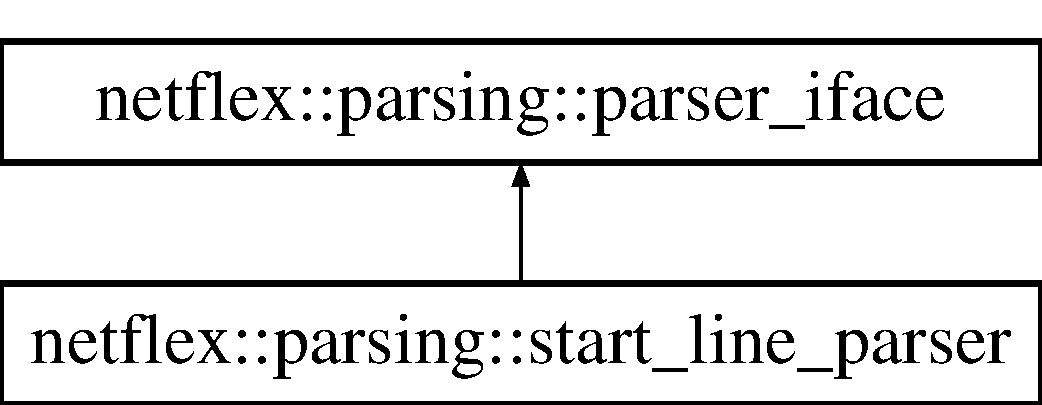
\includegraphics[height=2.000000cm]{classnetflex_1_1parsing_1_1start__line__parser}
\end{center}
\end{figure}
\subsection*{Public Member Functions}
\begin{DoxyCompactItemize}
\item 
\mbox{\Hypertarget{classnetflex_1_1parsing_1_1start__line__parser_a8a8554f0cfedc23f4955f5fcd4fa2a30}\label{classnetflex_1_1parsing_1_1start__line__parser_a8a8554f0cfedc23f4955f5fcd4fa2a30}} 
\hyperlink{classnetflex_1_1parsing_1_1start__line__parser_a8a8554f0cfedc23f4955f5fcd4fa2a30}{start\+\_\+line\+\_\+parser} (\hyperlink{classnetflex_1_1http_1_1request}{http\+::request} \&request)
\begin{DoxyCompactList}\small\item\em ctor \& dtor \end{DoxyCompactList}\item 
\mbox{\Hypertarget{classnetflex_1_1parsing_1_1start__line__parser_ae86a3442c52945efb4868c0853d89be7}\label{classnetflex_1_1parsing_1_1start__line__parser_ae86a3442c52945efb4868c0853d89be7}} 
\hyperlink{classnetflex_1_1parsing_1_1start__line__parser_ae86a3442c52945efb4868c0853d89be7}{start\+\_\+line\+\_\+parser} (const \hyperlink{classnetflex_1_1parsing_1_1start__line__parser}{start\+\_\+line\+\_\+parser} \&)=delete
\begin{DoxyCompactList}\small\item\em copy ctor \& assignment operator \end{DoxyCompactList}\item 
\mbox{\Hypertarget{classnetflex_1_1parsing_1_1start__line__parser_a38a89b7c84cfcf444a519920f45b1b7e}\label{classnetflex_1_1parsing_1_1start__line__parser_a38a89b7c84cfcf444a519920f45b1b7e}} 
\hyperlink{classnetflex_1_1parsing_1_1start__line__parser}{start\+\_\+line\+\_\+parser} \& {\bfseries operator=} (const \hyperlink{classnetflex_1_1parsing_1_1start__line__parser}{start\+\_\+line\+\_\+parser} \&)=delete
\item 
\mbox{\Hypertarget{classnetflex_1_1parsing_1_1start__line__parser_a663858012ee38e99d0c39444221bf4b5}\label{classnetflex_1_1parsing_1_1start__line__parser_a663858012ee38e99d0c39444221bf4b5}} 
\hyperlink{classnetflex_1_1parsing_1_1parser__iface}{parser\+\_\+iface} \& \hyperlink{classnetflex_1_1parsing_1_1start__line__parser_a663858012ee38e99d0c39444221bf4b5}{operator$<$$<$} (std\+::string \&)
\begin{DoxyCompactList}\small\item\em \hyperlink{classnetflex_1_1parsing_1_1parser__iface}{parser\+\_\+iface} impl \end{DoxyCompactList}\item 
\mbox{\Hypertarget{classnetflex_1_1parsing_1_1start__line__parser_a7b32cf1d39bfaa78d76dff258d984f95}\label{classnetflex_1_1parsing_1_1start__line__parser_a7b32cf1d39bfaa78d76dff258d984f95}} 
bool \hyperlink{classnetflex_1_1parsing_1_1start__line__parser_a7b32cf1d39bfaa78d76dff258d984f95}{is\+\_\+done} (void) const
\begin{DoxyCompactList}\small\item\em returns whether the given http packet section has been fully parsed \end{DoxyCompactList}\end{DoxyCompactItemize}
\subsection*{Additional Inherited Members}


\subsection{Detailed Description}
H\+T\+TP Start Line \href{https://tools.ietf.org/html/rfc7230#section-3.1}{\tt https\+://tools.\+ietf.\+org/html/rfc7230\#section-\/3.\+1}

start-\/line = request-\/line / status-\/line request-\/line = method SP request-\/target SP H\+T\+T\+P-\/version C\+R\+LF method = token 

The documentation for this class was generated from the following file\+:\begin{DoxyCompactItemize}
\item 
includes/netflex/parsing/start\+\_\+line\+\_\+parser.\+hpp\end{DoxyCompactItemize}

%--- End generated contents ---

% Index
\backmatter
\newpage
\phantomsection
\clearemptydoublepage
\addcontentsline{toc}{chapter}{Index}
\printindex

\end{document}
